\documentclass[
    oneside,
    10pt,
    language=italian,
    pagestyle=notes,
    fontstyle=palaeuler,
    thmstyle=margin-name
]{modernth}
    \usepackage{probability}
    \usepackage{pgfplots}

\pgfplotsset{
    compat=1.17,
    every axis/.append style={
        axis x line=middle,    % put the x axis in the middle
        axis y line=middle,    % put the y axis in the middle
        axis line style={->}, % arrows on the axis
        xlabel={$x$},          % default put x on x-axis
        ylabel={$y$},          % default put y on y-axis
    },
    cmhplot/.style={color=red,mark=none,line width=1pt},
    soldot/.style={color=red,only marks,mark=*},
    holdot/.style={color=red,fill=white,only marks,mark=*},
}

\tikzset{>=stealth}

\usetikzlibrary{external}
\tikzexternalize[prefix=figures/]

\begin{document}

\author{Luca De Paulis}
\title{Calcolo delle Probabilità e Statistica}
\maketitle

\frontmatter{}
\tableofcontents

\mainmatter{}
% CAPITOLO 1
\chapter{Statistica descrittiva}
\chapter{Statistica descrittiva}

\section{Concetti base}

La statistica descrittiva è la branca della statistica che descrive fenomeni statistici senza sfruttare nozioni di probabilità. I concetti fondamentali della statistica descrittiva sono il concetto di \emph{popolazione} e di \emph{campione}: la popolazione è l'insieme delle entità e dei dati che vogliamo studiare, mentre il campione è un piccolo sottoinsieme della popolazione che verrà analizzato per fini statistici.

Altri concetti base sono il concetto di \emph{frequenza assoluta} e \emph{relativa}: si dice frequenza assoluta di un evento $A$ il numero di volte che l'evento accade, senza considerare il numero di eventi (anche di tipo diverso) che accadono; invece si dice frequenza assoluta di un evento $A$ il numero di volte che l'evento accade diviso il numero di eventi totali.

\section{Analisi numerica dei dati}

Supponiamo di avere un vettore $\vec{x} = (x_1, \dots, x_n) \in \R^n$ che rappresenta i nostri dati. Possiamo definire alcune operazioni fondamentali su questi dati.

\begin{definition}
    [Media (empirica)] Dato $\vec x$ vettore di dati, si dice \emph{media (empirica)} il valore \begin{equation}
        \mean{x} \deq \frac{1}{n}\sum_{i=1}^n x_i = \frac{x_1 + \dots + x_n}{n}.
    \end{equation}
\end{definition}

Per descrivere quanto i dati contenuti in $\vec x$ si discostano dalla media $\mean x$ si usa il concetto di varianza:
\begin{definition}
    [Varianza] Dato $\vec x$ vettore di dati, si dice \emph{varianza campionaria} il valore \begin{equation}
        \var{\vec x} \deq \sum_{i=1}^n \frac{(x_i - \mean x)^2}{n-1};
    \end{equation} si dice invece \emph{varianza empirica} il valore \begin{equation}
        \var*{\vec x} \deq \sum_{i=1}^n \frac{(x_i - \mean x)^2}{n}.
    \end{equation}
\end{definition}

La varianza campionaria verrà usata quando i dati si riferiscono ad un campione, mentre la varianza empirica sarà più utile per trattare dati riferiti alle popolazioni.

In alcuni casi è utile conoscere la radice quadrata della varianza, quindi definiamo lo \emph{scarto quadratico medio} (o \emph{deviazione standard}) nel seguente modo: \begin{equation}
    \sd{\vec x} \deq \sqrt{\var{\vec x}}, \quad \sd*{\vec x} \deq \sqrt{\var*{\vec x}}.
\end{equation}

\begin{proposition}
    Vale la seguente uguaglianza: \begin{equation} \label{eq:uguaglianza_base}
        \sum_{i=1}^n (x_i - \mean x)^2 = \sum_{i=1}^n x_i^2 - n\mean{x}^2.
    \end{equation}
\end{proposition}
\begin{proof}
    \begin{align*}
        \sum_{i=1}^n (x_i - \mean x)^2 &= \sum_{i=1}^n (x_i^2 - 2x_i\mean x + \mean{x}^2)\\
        &= \sum_{i=1}^n x_i^2 - 2\mean x\sum_{i=1}^n x_i + \sum_{i=1}^n \mean{x}^2\\
        &= \sum_{i=1}^n x_i^2 - 2\mean x\sum_{i=1}^n x_i + n\mean{x}^2\\
        \intertext{Ricordando che $\mean x = \frac1n \sum_{i=1}^n x_i$, ovvero $\sum_{i=1}^n x_i = 2\mean x$:}
        &= \sum_{i=1}^n x_i^2 - 2n\mean{x}^2 + n\mean{x}^2\\
        &= \sum_{i=1}^n x_i^2 - n\mean{x}^2. \qedhere
    \end{align*}
\end{proof}

Usando la \eqref{eq:uguaglianza_base} otteniamo che \[
    \var*{\vec x} = \sum_{i=1}^n \frac{x_i^2}{n} - \mean x^2.
\]

\begin{proposition}
    Dato $\vec x$ vettore dei dati, la varianza (campionaria o empirica) di $\vec x$ è $0$ se e solo se \[
        x_1 = \dots = x_n = \mean x.    
    \]
\end{proposition}
La dimostrazione è ovvia: essendo la varianza definita come la somma di termini non negativi, essa è uguale a $0$ se e soltanto se ogni termine è uguale a $0$, ovvero se e solo se $x_i = \mean x$ per ogni $i = 1, \dots, n$. La varianza quindi rappresenta la "dispersione" dei dati: più è alta, più i dati sono diversi tra loro; più è bassa e più sono vicini (nel caso limite in cui sono tutti uguali la varianza è $0$).

Possiamo generalizzare questa idea: fissata una soglia $d \in \R$ consideriamo il numero di elementi $x_i$ la cui distanza dalla media $\mean x$ è maggiore o uguale a $d$: \[
    \#\set{x_1 \suchthat \abs*{x_i - \mean x} \geq d}.
\] È possibile dimostrare che vale la seguente disuguaglianza: \[
    \#\set{x_1 \suchthat \abs*{x_i - \mean x} \geq d} \leq \frac{1}{d}\sum_{i=1}^n (x_i - \mean x)^2,
\] da cui, dividendo entrambi i membri per $n$, segue un caso particolare della cosiddetta \emph{disuguaglianza di Chebyshev}: \begin{equation}
    \frac{\#\set{x_1 \suchthat \abs*{x_i - \mean x} \geq d}}{n} \leq \frac{\var*{\vec x}}{d}.
\end{equation} Il membro sinistro rappresenta la \emph{percentuale} dei dati che si discostano dalla media per un valore superiore alla soglia $d$.

Un altro metodo utile per ripartire i dati è utilizzare la cosiddetta \emph{funzione di ripartizione empirica}.
\begin{definition}
    Dato $\vec{x} \in \R^n$ vettore dei dati, la funzione di ripartizione empirica è una funzione $F_e : \R \to [0,1]$ tale che \begin{equation*}
        F_e(t) = \frac{\#\set{x_i \suchthat x_i \leq t}}{n}.
    \end{equation*}
\end{definition}
Dunque per ogni soglia $t$ la funzione di ripartizione empirica restituisce la percentuale dei dati che sono minori o uguali a $t$.

\begin{example}
    Se il vettore dei dati è $\vec x = (1.2, -0.7, 3.4, 1.6, 2.1)$ per trovare la funzione di ripartizione empirica $F_e$ mi conviene innanzitutto ordinarli, ottenendo \[
        \vec x = (-0.7, 1.2, 1.6, 2.1, 3.4).    
    \] A questo punto posso descrivere molto semplicemente la funzione di ripartizione empirica:
    \begin{itemize}
        \item se $t < -0.7$ allora $F_e(t) = 0$: tutti i dati sono maggiori della soglia $t$;
        \item se $t \in \halfCloseInt{-0.7, 1.2}$ allora $F_e(t) = \nicefrac{1}{5}$: un solo dato è sicuramente minore o uguale a $t$ (ovvero $x_1 = -0.7$), da cui dividendo per $n = 5$ si ottiene $\nicefrac{1}{5}$;
        \item se $t \in \halfCloseInt{1.2, 1.6}$ allora $F_e(t) = \nicefrac{2}{5}$: due dati sono minori o uguali a $t$ (ovvero $-0.7$ e $1.2$), da cui dividendo per $n = 5$ si ottiene $\nicefrac{2}{5}$;
        \item se $t \in \halfCloseInt{1.6, 2.1}$ allora $F_e(t) = \nicefrac{3}{5}$;
        \item se $t \in \halfCloseInt{2.1, 3.4}$ allora $F_e(t) = \nicefrac{4}{5}$;
        \item se $t \geq 3.4$ allora $F_e(t) = 1$ (tutti i dati sono minori o uguali a $t$, dunque la percentuale è $1$);
    \end{itemize}

    Il grafico di questa funzione è quindi:
    \begin{center}
        \begin{tikzpicture}
            \begin{axis}[
                width=380pt,
                ylabel=$F_e(t)$,
                xlabel=$t$,
                ymin=-0.3,ymax=1.3,
                xmin=-3,xmax=5,
                xtick = {-0.7,1.2,1.6,2.1,3.4},
                xticklabels = {$-0.7$,$1.2$,$1.6$,$2.1$,$3.4$},
                ytick = {0,0.2,0.6,0.8,0.4,1},
                yticklabels = {$0$,$0.2$,$0.6$,$0.8$,$0.4$,$1$},
            ] 
            \addplot[cmhplot, domain=-3:-0.7]{0};
            \addplot[cmhplot, domain=-0.7:1.2]{0.2};
            \addplot[cmhplot, domain=1.2:1.6]{0.4};
            \addplot[cmhplot, domain=1.6:2.1]{0.6};
            \addplot[cmhplot, domain=2.1:3.4]{0.8};
            \addplot[cmhplot, domain=3.4:7]{1};
            \addplot[holdot]coordinates{(-0.7,0)(1.2,0.2)(1.6,0.4)(2.1,0.6)(3.4,0.8)};
            \addplot[soldot]coordinates{(-0.7,0.2)(1.2,0.4)(1.6,0.6)(2.1,0.8)(3.4,1)};

                % \addplot[blue,smooth] {1/(1+exp(-x))};
                % \addlegendentry{Logistic sigmoid}
            \end{axis}
            
        \end{tikzpicture}
    \end{center}
\end{example}

\subsubsection{Percentili e quantili}
\begin{definition}
    [Percentile] Sia $k \in \R$ con $0 \leq k \leq 100$. Allora, dato un vettore dei dati $\vec x$ il $k$-esimo percentile è un qualsiasi numero $t \in \R$ tale che \begin{itemize}
        \item almeno $\nicefrac{k}{100}$ dei dati sono minori o uguali di $t$,
        \item almeno $\nicefrac{1-k}{100}$ dei dati sono maggiori o uguali a $t$.
    \end{itemize}
\end{definition}
Intuitivamente un numero reale $t$ è il $k$-esimo percentile del nostro vettore di dati $\vec x$ se $t$ è il più piccolo numero che è maggiore o uguale al $k$ percento dei dati. Dato che preferiamo trattare numeri compresi tra $0$ e $1$ invece che tra $0$ e $100$ introduciamo il concetto di $\beta$-quantile: se $t$ è un $k$-esimo percentile, allora $t$ è un $\beta$-quantile per $\beta = \nicefrac{k}{100}$.

Detto più direttamente, un numero $t$ è un $\beta$-quantile se \begin{itemize}
    \item almeno $\beta$ dei dati sono minori o uguali a $t$,
    \item almeno $1-\beta$ dei dati sono maggiori o uguali a $t$.
\end{itemize}

\begin{example}
    Dato il vettore $\vec x = (10, 20, 40, 60, 100)$, il dato $x_4 = 60$ corrisponde all'$80$-esimo percentile, o equivalentemente allo $0.80$-quantile.
\end{example}

Alcuni quantili particolari hanno dei nomi specifici:
\begin{itemize}
    \item lo $0.25$-quantile è anche chiamato \emph{primo quartile},
    \item lo $0.50$-quantile è anche chiamato \emph{mediana},
    \item lo $0.75$-quantile è anche chiamato \emph{terzo quartile}.
\end{itemize}

\subsubsection{Dati multipli}
In alcuni casi è necessario fare indagini statistiche su dati multipli: rappresentiamo i nostri dati come un vettore di coppie (o triple, o $n$-uple) di dati: \[
    (\vec x, \vec y) = ((x_1, y_1), \dots, (x_n, y_n)).    
\] Per studiare la \emph{correlazione} tra i dati delle $x$ e i dati delle $y$ abbiamo bisogno di alcuni strumenti:
\begin{definition}
    [Covarianza] Dato un vettore di coppie di dati $(\vec x, \vec y)$ si dice \emph{covarianza campionaria} il numero \begin{equation}
        \cov{\vec x, \vec y} \deq \frac{1}{n-1}\sum_{i=1}^n (x_i - \mean x)(y_i - \mean y);
    \end{equation} si dice invece \emph{convarianza empirica} il numero \begin{equation}
        \cov*{\vec x, \vec y} \deq \frac{1}{n}\sum_{i=1}^n (x_i - \mean x)(y_i - \mean y).
    \end{equation}
\end{definition}

\begin{definition}
    [Coefficiente di correlazione] Dato un vettore di coppie di dati $(\vec x, \vec y)$, se $\sd{\vec x}, \sd{\vec y} \neq 0$, si dice \emph{coefficiente di correlazione} il numero \[
        r(\vec x, \vec y) \deq \frac{\cov{\vec x, \vec y}}{\sd{\vec x}\sd{\vec y}} = \frac{\displaystyle\sum_{i=1}^n (x_i - \mean x)(y_i - \mean y)}{\displaystyle\sqrt{\sum_{i=1}^n (x_i-\mean x)^2}\sqrt{\sum_{i=1}^n (y_i-\mean y)^2}}.
    \]
\end{definition}

\begin{proposition}
    Dato un vettore di coppie di dati $(\vec x, \vec y)$ con $\sd{\vec x}, \sd{\vec y} \neq 0$, vale che \[
            0 \leq \abs[\big]{r(\vec x, \vec y)} \leq 1.
    \]
\end{proposition}
\begin{proof}
    Viene dalla disuguaglianza di Cauchy-Schwartz: \[
        \sum_{i=1}^n \abs[\big]{(x_i - \mean x)(y_i - \mean y)} \leq \sqrt{\sum_{i=1}^n (x_i-\mean x)^2}\sqrt{\sum_{i=1}^n (y_i-\mean y)^2},   
    \] da cui segue che \[
        \abs[\big]{r(\vec x, \vec y)} = \frac{\displaystyle\sum_{i=1}^n \abs[\big]{(x_i - \mean x)(y_i - \mean y)}}{\displaystyle\sqrt{\sum_{i=1}^n (x_i-\mean x)^2}\sqrt{\sum_{i=1}^n (y_i-\mean y)^2}} \leq 1. \qedhere
    \]
\end{proof}

Intuitivamente il coefficiente di correlazione misura quanto è semplice approssimare la relazione tra le $x$ e le $y$ con una funzione lineare affine, ovvero con una retta: per vedere ciò cerchiamo di capire quale retta approssima meglio i nostri dati.

Per approssimare linearmente $(\vec x, \vec y)$ dobbiamo fare in modo che la nostra retta $a + bx$ sia il più vicino possibile ai punti $(x_i, y_i)$ che formano i dati: vogliamo quindi che per ogni punto $x_i$ la distanza tra $y_i$ e $a+bx_i$ sia la minima possibile. Possiamo ottenere quello che vogliamo calcolando il seguente valore: \begin{equation}
    \min_{a, b \in \R^2} \sum_{i=1}^n (y_i - a - bx_i)^2.   \label{eq:min_dist_retta} 
\end{equation} (Eleviamo le distanze al quadrato in modo da renderle tutte positive e le sommiamo insieme poiché vogliamo che la distanza \emph{complessiva} della retta sia minima.)

\begin{theorem}
    Il valore minimo della quantità in \eqref{eq:min_dist_retta} si ottiene scegliendo \[
        b^\ast = \frac{\cov{\vec x, \vec y}}{\var{\vec x}}, \quad a^\ast = -b\mean x + \mean y.    
    \] Inoltre vale che \[
        \min_{a, b \in \R^2} \sum_{i=1}^n (y_i - a - bx_i)^2 = \sum_{i= 1}^n (y_i - \mean y)^2\left( 1 - r(\vec x, \vec y)^2 \right).
    \]
\end{theorem}
\begin{proof}
    ["Dimostrazione"] Sia $Q : \R^2 \to \R$ la funzione definita da \[
        Q(a, b) \deq \sum_{i=1}^n (y_i - a - bx_i)^2.
    \] Per dimostrare che questa funzione ha minimo calcoliamo i limiti all'infinito: siccome vale che \[
        \lim_{\abs a, \abs b \to +\infty} \sum_{i=1}^n (y_i - a - bx_i)^2 = +\infty    
    \] per il teorema di Weierstrass generalizzato questa funzone ha minimo. Per calcolarlo, imponiamo che le derivate parziali $\dfrac{\partial Q}{\partial a}$ e $\dfrac{\partial Q}{\partial b}$ siano uguali a $0$, da cui ricaviamo le espressioni per $a^\ast$ e $b^\ast$. Sostituendole in $Q$ otteniamo l'espressione per il minimo di $Q$, che è la seconda parte della tesi.
\end{proof}

La retta $a^\ast + b^\ast x$ viene detta \emph{retta di regressione} ed è la funzione lineare affine che meglio approssima i dati che abbiamo a nostra disposizione. Dato che la minima distanza tra la retta e il vettore dei dati (nel senso dato dalla formulazione in \eqref{eq:min_dist_retta}) è proporzionale a $\left(1 - r(\vec x, \vec y)^2\right)$, avremo che: \begin{itemize}
    \item più $r(\vec x, \vec y)^2$ si avvicina a $1$, più la distanza minima si avvicina a $0$ e quindi i dati sono correlati linearmente;
    \item più $r(\vec x, \vec y)^2$ si avvicina a $0$, più la distanza minima cresce e quindi i dati sono dispersi e non seguono una correlazione lineare.
\end{itemize}
Inoltre il coefficiente angolare della retta di regressione $b^\ast$ può essere riscritto come \[
    b^\ast = \frac{\cov{\vec x, \vec y}}{\var{\vec x}} = \frac{\cov{\vec x, \vec y}}{\sd{\vec x}\sd{\vec y}}\frac{\sd{\vec x}\sd{\vec y}}{\var{\vec x}} = r(\vec x, \vec y)\frac{\sd{\vec x}\sd{\vec y}}{\var{\vec x}}.
\] Dato che $\frac{\sd{\vec x}\sd{\vec y}}{\var{\vec x}} \geq 0$ il segno del coefficiente angolare dipende solamente dal coefficiente di correlazione: \begin{itemize}
    \item se $r(\vec x, \vec y) > 0$ la retta di regressione ha coefficiente angolare positivo, dunque è crescente e al crescere delle $x$ tendenzialmente crescono anche le $y$;
    \item se $r(\vec x, \vec y) < 0$ la retta di regressione ha coefficiente angolare negativo, dunque è decrescente e al crescere delle $x$ tendenzialmente le $y$ decrescono.
\end{itemize}

Il coefficiente di correlazione dunque ci dice quanto sono correlate le due quantità che stiamo esaminando (più è vicino ad $1$ e più sono correlate) e se al crescere della prima cresce anche la seconda (se è di segno positivo), oppure al crescere della prima la seconda diminuisce (se è di segno negativo).

% CAPITOLO 2
\chapter{Probabilità}
\chapter{Probabilità}

\section{Spazio di probabilità}

\begin{definition}
    [Algebra delle parti]
    Sia $\Omega$ un insieme. Una famiglia $\FF$ di sottoinsiemi di $\Omega$ si dice \emph{algebra delle parti su $\Omega$} se valgono le seguenti proprietà: \begin{enumerate}[label={(\roman*)}]
        \item $\varnothing, \Omega \in \FF$;
        \item se $A \in \FF$ allora $A\compl \in \FF$;
        \item se $A, B \in \FF$ allora $A \union B \in \FF$, $A \inters B \in \FF$.
    \end{enumerate}
\end{definition}

Un'algebra di parti su $\Omega$ modella bene l'insieme dei possibili eventi: \begin{enumerate}[label={(\roman*)}]
    \item l'insieme vuoto è un evento, ed in particolare corrisponde all'evento "non accade nessuno degli eventi nel nostro universo";
    \item l'insieme universo è un evento, ed in particolare corrisponde all'evento "accade una cosa qualsiasi nel nostro universo";
    \item se $A$ è un evento, allora $A\compl$ corrisponde all'evento "non accade $A$";
    \item se $A, B$ sono eventi, allora $A \union B$ corrisponde all'evento "accade $A$ oppure accade $B$";
    \item se $A, B$ sono eventi, allora $A \inters B$ corrisponde all'evento "accadono sia $A$ che $B$".
\end{enumerate}

\begin{definition}
    [Probabilità]
    Sia $\Omega$ un insieme e $\FF$ un'algebra delle parti su $\Omega$. Si dice \emph{probabilità} una funzione \[
        \P : \FF \to \interval[{0, 1}]  
    \] tale che \begin{enumerate}
        % [label={(\roman*)}]
        \item $\Prob{\Omega} = 1$,
        \item \label{def:prob_finit_add} $\P$ è \emph{finitamente additiva}: per ogni $A, B \in \FF$ disgiunti (ovvero $A \inters B = \varnothing$) vale che \[
            \Prob{A \union B} = \Prob{A} + \Prob{B}.
        \]
    \end{enumerate}
\end{definition}

% Questa definizione di probabilità è particolarmente intuitiva: la probabilità che accada l'evento $\Omega$ (ovvero che accada un evento qualsiasi) è $1$; invece se sappiamo che due eventi 

\begin{proposition}[Proprietà della probabilità]
    \label{prop:prop_probabil}
    Sia $\Omega$ un insieme e $\FF$ un'algebra delle parti su $\Omega$. Allora la funzione probabilità $\P$ soddisfa le seguenti proprietà:
    \begin{enumerate}
        \item $\Prob{\varnothing} = 0$;
        \item $\Prob{A\compl} = 1 - \Prob{A}$;
        \item se $B \subseteq A$ allora $\Prob{A \setminus B} = \Prob{A} - \Prob{B}$;
        \item per ogni $A, B \in \FF$ vale il \emph{principio di inclusione-esclusione}: \[
            \Prob{A \union B} = \Prob{A} + \Prob{B} - \Prob{A \inters B}.    
        \]
    \end{enumerate}
\end{proposition}
\begin{proof}
    Dimostriamo le quattro affermazioni separatamente: \begin{enumerate}
        \item Siccome \begin{itemize}
            \item $\varnothing \inters \varnothing = \varnothing$,
            \item $\varnothing \union \varnothing = \varnothing$,
            \item la funzione probabilità è \hyperref[def:prob_finit_add]{finitamente additiva}
        \end{itemize} segue che \[
            \Prob{\varnothing} = \Prob{\varnothing \union \varnothing} = \Prob{\varnothing} + \Prob{\varnothing}, 
        \] da cui, sottraendo $\Prob{\varnothing}$ ad entrambi i membri, otteniamo $\Prob{\varnothing} = 0$.
        \item Per definizione di complementare segue che $\Omega = A \union A\compl$. Inoltre un insieme e il suo complementare sono sempre disgiunti, dunque vale l'\hyperref[def:prob_finit_add]{additività finita}: \[
            1 = \Prob{\Omega} = \Prob{A \union A\compl} = \Prob{A} + \Prob{A\compl}    
        \] da cui segue che $\Prob{A\compl} = 1 - \Prob{A}$.
        \item Siccome $B \subseteq A$ possiamo scrivere $A = B \union (A \setminus B)$. Inoltre $B$ e $A \setminus B$ sono ovviamente disgiunti, dunque vale l'\hyperref[def:prob_finit_add]{additività finita}: \[
            \Prob{A} = \Prob[\big]{B \union (A \setminus B)} = \Prob{B} + \Prob{A \setminus B}   
        \] da cui segue che $\Prob{A \setminus B} = \Prob{A} - \Prob{B}$.
        \item Separiamo gli insiemi $A$ e $B$ in tre sottoinsiemi particolari: \begin{itemize}
            \item $C_1 = A \setminus (A \inters B)$, ovvero $C_1$ contiene solo gli elementi che sono in $A$ e non in $B$,
            \item $C_2 = B \setminus (A \inters B)$, ovvero $C_2$ contiene solo gli elementi che sono in $B$ e non in $A$,
            \item $C_3 = A \inters B$, ovvero $C_3$ contiene tutti e soli gli elementi che appartengono sia ad $A$ che a $B$.
        \end{itemize}
        Notiamo che \begin{itemize}
            \item $A \union B = C_1 \union C_2 \union C_3$,
            \item $A = C_1 \union C_3$, $B = C_2 \union \C_3$,
            \item i tre insiemi $C_1, C_2, C_3$ sono tutti e tre disgiunti.
        \end{itemize} Dunque per additività finita:
        \begin{align*}
            \Prob{A \union B} &= \Prob{C_1 \union C_2 \union C_3}\\
            &= \Prob{C_1} + \Prob{C_2 \union C_3}
            \intertext{Aggiungiamo e sottraiamo $\Prob{C_3}$:}
            &= \Prob{C_1} + \Prob{C_2 \union C_3} + \Prob{C_3} - \Prob{C_3}\\
            &= \Prob{C_1 \union C_3} + \Prob{C_2 \union C_3} - \Prob{C_3}\\
            \intertext{Infine, siccome $C_1 \union C_3 = A$, $C_2 \union C_3 = B$, $C_3 = A \inters B$:}
            &= \Prob{A} + \Prob{B} - \Prob{A \inters B}. \qedhere   
        \end{align*}
    \end{enumerate}
\end{proof}

Questa formalizzazione dei concetti di evento e probabilità è però limitata: possiamo calcolare la probabilità di unioni e intersezioni di un numero finito di eventi, ma non di un numero infinito (anche se numerabile). Abbiamo quindi bisogno di un'estensione di questi concetti che ci permetta di "andare al limite".

\begin{definition}[Sigma-algebra]
    Sia $\Omega$ un insieme. Una famiglia $\FF$ di sottoinsiemi di $\Omega$ si dice \emph{$\sigma$-algebra su $\Omega$} se valgono le seguenti proprietà: 
    \begin{enumerate}[label={(\roman*)}]
        \item $\varnothing, \Omega \in \FF$;
        \item se $A \in \FF$ allora $A\compl \in \FF$;
        \item se $\parens*{A_n}_{n\in\N}$ è un insieme numerabile di elementi di $\FF$ (ovvero per ogni $n \in \N$ vale che $A_n \in \FF$), allora \[
            \bigunion_{n = 1}^{\infty} A_n \in \FF, \quad \biginters_{n = 1}^{\infty} A_n \in \FF.    
        \]
    \end{enumerate}
\end{definition}

\begin{definition}
    [Probabilità]
    Sia $\Omega$ un insieme e $\FF$ una $\sigma$-algebra su $\Omega$. Si dice \emph{probabilità} una funzione \[
        \P : \FF \to \interval[{0,1}]    
    \] tale che \begin{enumerate}[label={(\roman*)}]
        \item $\Prob{\Omega} = 1$,
        \item \label{def:prob_numerab_add} $\P$ è \emph{numerabilmente additiva}: data una successione $(A_n)_{n\in\N}$ a valori in $\FF$ (ovvero con $A_i \in \FF$ per ogni $i \in \N$) a due a due disgiunti (ovvero $A_i \inters A_j = \varnothing$ per ogni $i \neq j$) vale che \[
            \Prob*{\bigunion_{n = 1}^{\infty} A_n} 
            = \sum_{n = 1}^{\infty} \Prob{A_i}.
        \]
    \end{enumerate}
\end{definition}

\begin{remark}
    Questa nuova definizione di probabilità è un'\emph{estensione} della definizione iniziale: infatti dalla additività numerabile segue necessariamente l'additività finita.
\end{remark}
\begin{proof}
    Siano $A, B \in \FF$ disgiunti. Allora possiamo costruire la successione \[
        C_n \deq \begin{cases}
            A, &\text{se } n = 1, \\
            B, &\text{se } n = 2, \\
            \varnothing, &\text{altrimenti.}
        \end{cases}
    \] Gli insiemi che formano questa successione sono a due a due disgiunti, in quanto $A$ e $B$ sono disgiunti e l'intersezione tra un insieme qualunque e l'insieme vuoto è sempre vuota.

    Inoltre l'unione di tutti questi insiemi è uguale all'unione di $A$ e $B$, da cui segue che \begin{align*}
        \Prob*{A \union B} &= \Prob*{\bigunion_{n = 1}^\infty C_n} \tag{per addit. num.}\\
        &= \sum_{i=1}^\infty \Prob{C_n} \\
        &= \Prob{C_1} + \Prob{C_2} + \sum_{i=3}^\infty \Prob{C_n}\\
        \intertext{Siccome $C_n = \varnothing$ per ogni $n \geq 3$ e la probabilità dell'insieme vuoto è $0$ la sommatoria vale $0$ e dunque segue che}
        &= \Prob{C_1} + \Prob{C_2}\\
        &= \Prob{A} + \Prob{B}
    \end{align*} cioè la funzione probabilità è finitamente additiva.
\end{proof}
\begin{remark}
    Dato che la probabilità estesa è finitamente additiva, continua a valere la \autoref{prop:prop_probabil}.
\end{remark}

\begin{definition}
    [Spazio di probabilità] Sia $\Omega$ un insieme, $\FF$ una $\sigma$-algebra su $\Omega$ e $\P$ una funzione probabilità definita su $\FF$: la tripla $(\Omega, \FF, \P)$ si dice \emph{spazio di probabilità}.
\end{definition}

\begin{definition}
    [Eventi trascurabili e quasi certi] Sia $(\Omega, \FF, \P)$ uno spazio di probabilità. Un evento $A \in \FF$ si dice \begin{itemize}
        \item \emph{trascurabile} se $\Prob{A} = 0$;
        \item \emph{quasi certo} se $\Prob{A} = 1$.
    \end{itemize}
\end{definition}

La definizione "estesa" di probabilità ci consente di "passare al limite", ovvero di calcolare in modo semplice la probabilità di un evento definito come unione o intersezione numerabile di eventi.

\begin{proposition}
    Sia $(\Omega, \FF, \P)$ uno spazio di probabilità e sia \[
        A_1 \subseteq A_2 \subseteq A_3 \subseteq \dots    
    \] una catena di insiemi, con $A_i \in \FF$ per ogni $i \in \N$. Sia inoltre \[
        A \deq \bigunion_{i=1}^\infty A_i.    
    \] Allora vale che \begin{equation}
        \Prob{A} = \lim_{n \to +\infty} \Prob{A_n}.
    \end{equation}
\end{proposition}
\begin{proof}
    Definiamo $B_1 = A_1$, $B_n = A_n \setminus A_{n-1}$. L'unione di queste due successioni di insiemi è la stessa: \[
        \bigunion_{i=1}^\infty B_i = \bigunion_{i=1}^\infty A_i.    
    \] Dalla definizione di $B_n$ e dalla \autoref{prop:prop_probabil} (in particolare dal terzo punto, siccome $A_{n-1} \subseteq A_n$) segue che \[
        \Prob{B_n} = \Prob{A_n \setminus A_{n-1}} = \Prob{A_n} - \Prob{A_{n-1}}.
    \] Inoltre i $B_n$ sono a due a due disgiunti, dunque vale l'\hyperref[def:prob_numerab_add]{additività numerabile}: \begin{align*}
        \Prob{A} &= \Prob*{\bigunion_{i=1}^\infty A_i} \\
        &= \Prob*{\bigunion_{i=1}^\infty B_i}\\
        &= \sum_{i=1}^\infty \Prob{B_n}\\
        &= \lim_{n\to +\infty} \sum_{i=1}^n \Prob{B_i}\\
        &\begin{aligned}
            \ = \lim_{n \to +\infty} &\Prob{B_1} + \Prob{B_2} + \dots \\
            &+ \Prob{B_{n-1}} + \Prob{B_n}\\
        \end{aligned}\\
        &\begin{aligned}
            \ = \lim_{n \to +\infty} &\Prob{A_1} + (\Prob{A_2} - \Prob{A_1}) + \dots\\
            &+ (\Prob{A_{n-1}} - \Prob{A_{n-2}})\\
            &+ (\Prob{A_{n}} - \Prob{A_{n-1}})
        \end{aligned}\\
        &= \lim_{n \to +\infty} \Prob{A_n}. \qedhere
    \end{align*}
\end{proof}

\paragraph{Insieme fondamentale finito} Nel caso in cui $\Omega$ sia un insieme finito possiamo scriverlo come \[
    \Omega \deq \set{w_1, \dots, w_n}    
\] dove $n$ è la cardinalità di $\Omega$. Come $\sigma$-algebra su $\Omega$ possiamo sempre prendere l'insieme delle parti $\PP(\Omega)$, ovvero l'insieme di tutti i sottoinsiemi di $\Omega$: in questo modo tutti i sottoinsiemi di $\Omega$ sono eventi.

Chiamiamo $p_i$ la probabilità che accada l'evento $\set{w_i} \in \PP(\Omega)$, ovvero \[
    p_i \deq \Prob[\big]{\set{w_i}}.    
\] Sicuramente $p_i \geq 0$ (in quanto la funzione probabilità restituisce numeri reali tra $0$ e $1$); inoltre vale che \[
    \sum_{i=1}^n p_i = p_1 + p_2 + \dots + p_n = 1.    
\] Infatti: \begin{align*}
    p_1 + p_2 + \dots + p_n &= \Prob[\big]{\set{w_1}} + \Prob[\big]{\set{w_2}} + \dots + \Prob[\big]{\set{w_n}}\\
    &= \Prob[\big]{\set{w_1} \union \set{w_2} \union \dots \union \set{w_n}}\\
    &= \Prob[\big]{\set{w_1, w_2, \dots, w_n}}\\
    &= \Prob{\Omega}\\
    &= 1.
\end{align*}

Se $\Omega$ è finito e tutti gli eventi sono circa equiprobabili si può prendere \[
    p_i = \frac1n.    
\] In questo caso si parla di \emph{distribuzione uniforme di probabilità}. Dato un evento $A \in \PP(\Omega)$, nel caso di distribuzione uniforme, si ha che \[
    \Prob{A} = \frac{\#A}{\#\Omega} = \frac{\#\text{casi favorevoli}}{\#\text{casi totali}}.   
\]
\section{Probabilità condizionata}

\begin{example}
    Immaginiamo di star giocando alla roulotte e sappiamo che è appena uscito un numero pari. Qual è la probabilità che questo numero sia $4$?
    
    Sia $A$ l'evento "è uscito $4$" e sia $B$ l'evento "è uscito un numero pari". Siccome sappiamo che è uscito un numero pari, e i numeri pari alla roulotte sono $18$, la probabilità che sia uscito proprio $4$ (sapendo che il numero uscito è pari) equivale a $\nicefrac{1}{18}$.

    Possiamo tuttavia pensarla in questo modo: $\nicefrac{1}{18}$ è la probabilità che gli eventi $A$ e $B$ accadano contemporaneamente (ovvero è la probabilità di $A \inters B$) diviso la probabilità che sia avvenuto l'evento $B$: \[
        \frac{1}{18} = \frac{\Prob{A \inters B}}{\Prob{B}} = \frac{\nicefrac{1}{37}}{\nicefrac{18}{37}}.    
    \]
\end{example}

\begin{definition}
    [Probabilità condizionata] Sia $(\Omega, \FF, \P)$ uno spazio di probabilità e sia $B \in \FF$ non trascurabile. Si dice \emph{probabilità di $A$ condizionata a $B$} la quantità \[
        \Prob{A \given B} =  \frac{\Prob{A \inters B}}{\Prob{B}}.   
    \]
\end{definition}

\begin{remark}
    La funzione $\P^\prime : \FF \to \interval[{0, 1}]$ data da \[
        \P^\prime(A) \deq \Prob{A \given B}    
    \] è una probabilità.
\end{remark}

\begin{proposition}
    [Formula di Bayes] Siano $A, B$ due eventi non trascurabili. Allora vale che \[
        \Prob{B \given A} = \frac{\Prob{A \given B}\Prob{B}}{\Prob{A}}.    
    \]
\end{proposition}
\begin{proof}
    Per definizione di probabilità condizionata \[
        \Prob{A \given B}\Prob{B} = \Prob{A \inters B} = \Prob{B \given A}\Prob{A},    
    \] da cui la tesi.
\end{proof}

\begin{proposition}
    [Formula del condizionamento ripetuto]
    Siano $A_1, \dots, A_n$ eventi non trascurabili. Allora \[
        \Prob{A_1 \inters \dots \inters A_n} = \Prob{A_1}\Prob{A_2 \given A_1}\cdots \Prob{A_n \given A_{n-1} \inters \dots \inters A_1}.    
    \]
\end{proposition}
\begin{proof}
    Per definizione di probabilità condizionata \begin{align*}
        &\Prob{A_1}\Prob{A_2 \given A_1}\cdots \Prob{A_n \given A_{n-1} \inters \dots \inters A_1}\\
        = {}&{}\Prob{A_1}
        \frac{\Prob{A_1 \inters A_2}}{\Prob{A_1}}
        \frac{\Prob{A_3 \inters A_2 \inters A_1}}{\Prob{A_2 \inters A_1}}
        \cdots 
        \frac{\Prob{A_n \inters \dots \inters A_1}}{\Prob{A_{n-1} \inters \dots \inters A_1}}\\
        = {}&{}\Prob{A_1 \inters \dots \inters A_n}. \qedhere
    \end{align*}
\end{proof}

\begin{definition}
    [Sistema di alternative]
    Sia $(\Omega, \FF, \P$ uno spazio di probabilità e siano $B_1, \dots, B_n \in \FF$. Allora se $B_1, \dots, B_n$ formano una partizione di $\Omega$ (ovvero la loro unione è $\Omega$ e la loro intersezione a due a due è vuota) si dice che $B_1, \dots, B_n$ è un \emph{sistema di alternative}.
\end{definition}
\begin{remark}
    Un sistema di alternative non è necessariamente finito: data una famiglia numerabile $(B_i)_{i \in \N}$ di sottoinsiemi di $\Omega$, essa rappresenta un sistema di alternative se è una partizione di $\Omega$.
\end{remark}

\begin{proposition}
    [Formula di fattorizzazione]
    Sia $B_1, \dots, B_n$ un sistema di alternative e $A \in \FF$ un evento. Allora vale che \[
        \Prob{A} = \sum_{i = 1}^n \Prob{A \given B_i}\Prob{B_i}.    
    \]
\end{proposition}

\begin{proposition}
    [Formula delle probabilità delle cause]
    Sia $B_1, \dots, B_n$ un sistema di alternative e $A \in \FF$ un evento. Allora per ogni $i \in \set{1, \dots, n}$ vale che \[
        \Prob{B_i \given A} = \frac{\Prob{A \given B_i}\Prob{B_i}}{\Prob{A}}.    
    \]
\end{proposition}

\section{Indipendenza stocastica}

Vogliamo rendere l'idea che talvolta conoscere se un evento $A$ si è verificato oppure no non influenza la probabilità che l'evento $B$ si verifichi e viceversa. Sfruttando le probabilità condizionate, possiamo esprimerlo con una di queste due formule: \begin{align*}
    &(1):\; \Prob{B \given A} = \Prob{A}. &(2):\; \Prob{A \given B} = \Prob{A}.
\end{align*}

È facile dimostrare che queste due condizioni sono equivalenti; tuttavia nessuna delle due modella precisamente la nostra condizione, poiché non sono simmetriche e richiedono che $A$ e $B$ siano non trascurabili.

\begin{definition}
    [Indipendenza stocastica] Siano $A, B \in \FF$ due eventi. Allora $A$ e $B$ sono indipendenti stocasticamente se \[
        \Prob{A \inters B} = \Prob{A}\Prob{B}.    
    \]
\end{definition}

\begin{proposition}
    [Conseguenze dell'indipendenza stocastica] Sia $(\Omega, \FF, \P$ uno spazio di probabilità e siano $A, B$ due eventi. Valgono le seguenti affermazioni.
    \begin{enumerate}
        \item Se $A, B$ sono indipendenti, allora $A\compl$ e $B$ sono indipendenti.
        \item Se $A$ è trascurabile oppure quasi certo, allora $A$ e $B$ sono indipendenti qualunque sia $B$.
        \item Se $A$ e $B$ sono non trascurabili e incompatibili (ovvero $A \inters B = \varnothing$) allora $A$ e $B$ non sono indipendenti.
    \end{enumerate}
\end{proposition}
\begin{proof}
    Mostriamo le tre affermazioni separatamente.
    \begin{enumerate}
        \item Mostriamo che $A\compl$ e $B$ sono indipendenti tramite la definizione: \begin{align*}
            \Prob{A\compl \inters B} &= \Prob{B \setminus (A \inters B)}  \tag{per la \ref{prop:prop_probabil}}\\
            &= \Prob{B} - \Prob{A \inters B} \tag{$A, B$ indip.}\\
            &= \Prob{B} - \Prob{A}\Prob{B}\\
            &= \Prob{B}(1 - \Prob{A})\\
            &= \Prob{B}\Prob{A\compl}.
        \end{align*}
        \item Sia $B$ un evento qualunque: allora se $A$ è quasi certo segue che \[
            \Prob{A \inters B} = \Prob{A \given B}\Prob{B} = 1 \cdot \Prob{B} = \Prob{A}\Prob{B}.    
        \] Dimostrazione analoga se $A$ è trascurabile.
        \item Se $A \inters B = \varnothing$ allora $\Prob{A \inters B} = \Prob{\varnothing} = 0$, dunque se fossero indipendenti avremmo che $\Prob{A}\Prob{B} = 0$, il che è assurdo poiché li abbiamo supposti entrambi non trascurabili. \qedhere
    \end{enumerate}
\end{proof}
\section{Probabilità sulla retta reale}

Se il nostro insieme $\Omega$ è l'insieme $\R$ dei numeri reali, possiamo definire diversi tipi di probabilità.

\subsubsection{Probabilità discreta}
Il primo tipo di probabilità che possiamo definire su $\R$ è la \emph{probabilità discreta}: dato un insieme finito o numerabile di punti $(x_i)_{i \in \N}$ poniamo \[
    p(x_i) \deq \Prob{\set{x_i}}.    
\] Siccome vogliamo definire la nostra probabilità in modo che questi sottoinsiemi siano gli unici non trascurabili, imponiamo inoltre che \[
    \sum_{i \in \N} p(x_i) = 1.    
\] 

La probabilità è quindi \emph{concentrata} in un insieme numerabile di punti: dato $A \subseteq \R$ la probabilità dell'insieme $A$ è \[
    \Prob{A} = \sum_{x_i \in A} p(x_i).    
\]

\begin{definition}[Funzione di massa]
    La funzione $p : \R \to \R$ tale che \[
        p(x) \deq \begin{cases}
            \Prob{\set{x_i}} &\text{se } x = x_i \text{ per qualche } x_i\\
            0 &\text{altrimenti}
        \end{cases}    
    \]  è detta \emph{funzione di massa} oppure \emph{densità discreta}.
\end{definition}

\begin{remark}
    Una probabilità discreta può essere definita su ogni sottoinsieme di $\R$: come vedremo, questo non è il caso per altri tipi di probabilità.
\end{remark}

\subsubsection{Probabilità definita da una densità}

\begin{definition}
    [Densità di probabilità]
    Si dice \emph{densità di probabilità} una funzione $f : \R \to \interval[{0, +\infty})$ integrabile e tale che \[
        \int_{-\infty}^{+\infty} f(x)dx = 1.    
    \]
\end{definition}

\begin{definition}
    [Probabilità definita da una densità]
    Sia $f : \R \to \interval[{0, +\infty})$ una densità, $A \subseteq \R$. La probabilità definita da $f$ è tale che \[
        \Prob{A} = \int_{A} f(x)dx.    
    \]
\end{definition}

Notiamo che questa funzione definisce davvero una probabilità:
\begin{itemize}
    \item la probabilità di tutto $\R$ è \[
        \Prob{\R} = \int_{\R} f(x)dx = \int_{-\infty}^{+\infty} f(x)dx = 1.    
    \]
    \item è finitamente additiva: se $A, B \subseteq \R$ sono disgiunti, allora \[
        \Prob{A \union B} = \int_{A \union B} f(x)dx = \int_A f(x)dx + \int_B f(x)dx = \Prob{A} + \Prob{B}.    
    \]
    \item è anche numerabilmente additiva (deriva dal Teorema di Beppo-Levi).
\end{itemize}

Tuttavia questa probabilità, al contrario della probabilità discreta, non è definibile su tutti i sottoinsiemi di $\R$.
\begin{example}
    Supponiamo di volere una funzione che restituisce un numero reale a caso tra $0$ e $1$.

    Lo spazio di probabilità più naturale per questa funzione è $\Omega = \interval[{0, 1}]$, in quanto sicuramente il numero scelto sarà in questo intervallo. Per definire la probabilità di un sottoinsieme di $\Omega$, iniziamo studiando il caso in cui il sottoinsieme sia un intervallo chiuso $\interval[{a, b}]$.

    La probabilità che un numero casuale sia in $\interval[{a, b}]$ può essere pensata come la lunghezza dell'intervallo $\interval[{a, b}]$ diviso la lunghezza dello spazio universo $\Omega$: dunque \[
        \Prob{\interval[{a, b}]} = \frac{b - a}{1} = b - a.    
    \]

    Questa probabilità può essere definita come \emph{probabilità data da una densità}: la densità ad essa relativa è la funzione \[
        f(x) \deq \begin{cases}
            1 &\text{se } 0 \leq x \leq 1\\
            0 &\text{altrimenti}.
        \end{cases}    
    \]

    Questo esempio innanzitutto mostra la differenza tra \emph{eventi trascurabili} e \emph{eventi impossibili}: preso un qualunque $x \in \interval[{0, 1}]$ si ha che \[
        \set{x} \subseteq \interval*[{x - \frac1n, x + \frac{1}{n}}],    
    \] qualunque sia $n \in \N$. Questo significa che la probabilità del singoletto $\set{x}$ deve essere minore o uguale della probabilità dell'insieme in cui è contenuto, ovvero \[
        \Prob{\set{x}} \leq \Prob*{\interval*[{x - \frac1n, x + \frac1n}]} = \frac2n,    
    \] ma siccome ciò deve valere per $n$ arbitrariamente grande segue che $\Prob{\set x} = 0$. L'evento definito da $\set{x}$ è quindi trascurabile, ma certamente non è impossibile in quanto $x$ può essere il risultato dell'estrazione di un numero reale casuale.

    Il secondo punto, molto più difficile da mostrare, è che questa probabilità non è definita per ogni sottoinsieme di $\R$, ma solo per i sottoinsiemi \emph{misurabili}: il \emph{controesempio di Vitali} mostra che esistono sottoinsiemi di $\interval[{0, 1}]$ per cui questa probabilità non può essere definita. 
\end{example} 

D'ora in avanti considereremo soltanto sottoinsiemi misurabili di $\R$.

\paragraph{Densità esponenziale} Un tipo di densità molto utile è quella definita dalla seguente funzione: \[
    f(x) = \begin{cases}
        e^{-x} &\text{se } x \geq 0\\
        0 &\text{altrimenti.}
    \end{cases}    
\] Questa funzione è una probabilità in quanto è integrabile e \begin{align*}
    \int_{-\infty}^{+\infty} f(x)dx &= \int_{-\infty}^0 0dx + \int_0^{+\infty} e^{-x} \\
    = &\lim_{M \to +\infty} \left[ -e^{-x} \right]_0^M \\
    % = &\parens*{\lim_{M \to +\infty} -e^{-x}} + 1 \\
    = &\lim_{M \to +\infty} -e^{-x} + 1 \\
    = &1.
\end{align*}
\section{Variabili aleatorie}

Per introdurre il concetto di variabili aleatorie e la loro utilità useremo il seguente esempio:
\begin{example}
    Supponiamo di giocare alla roulotte e di aver puntato 1£ sul numero $28$ e 1£ sull'uscita di un numero pari. Possiamo ad esempio domandarci quanto sia la probabilità di vincere più di 10£, oppure quanto sia la probabilità di perdere soldi.

    Lo spazio più naturale per questo problema è l'insieme dei possibili risultati della roulotte, ovvero $\Omega = \set{0, 1, \dots, 36}$ munito della distribuzione uniforme di probabilità; tuttavia gli eventi che vogliamo considerare ("vincere più di 10£", "perdere soldi") non sono sottoinsiemi di $\Omega$, bensì di $\R$.
    
    Possiamo quindi definire una funzione $X : \Omega \to \R$ che indichi nel seguente modo la "vittoria netta": \[
        X(\omega) = \begin{cases}
            36, &\text{se } \omega = 28\\
            0, &\text{se } \omega \neq 28, \omega \text{ è pari}\\
            -1, &\text{se } \omega = 0\\
            -2, &\text{se } \omega \text{ è dispari}.\\
        \end{cases}  
    \]
    Usando la funzione $X$ possiamo \emph{trasportare} la probabilità da $\Omega$ a $\R$: la risposta alla prima domanda è dunque \[
        \Prob[\big]{\set{\omega \in \Omega \given X(\omega) > 10}} 
        = \Prob*{X^{-1}\parens[\big]{\interval({10, +\infty})}} 
        = \frac{1}{37};    
    \] la risposta alla seconda domanda è invece \[
        \Prob[\big]{\set{\omega \in \Omega \given X(\omega) < 0}} 
        = \Prob*{X^{-1}\parens[\big]{\interval({-\infty, 0})}} 
        = \frac{19}{37}.    
    \]
\end{example}

\begin{definition}
    [Variabili aleatorie] Sia $(\Omega, \FF, \P)$ uno spazio di probabilità. Una funzione $X : \Omega \to \R$ si dice \emph{variabile aleatoria} e la funzione dall'insieme dei \emph{sottoinsiemi misurabili di $\R$} in $\interval[{0, 1}]$ definita da \[
        \Prob_{X}{A} \deq \Prob*{X\inv(A)}  
    \] viene detta \emph{legge di probabilità} associata alla variabile aleatoria $X$.
\end{definition}

\begin{remark}
    Non definiamo cosa sia un sottoinsieme misurabile di $\R$, ma la maggior parte degli insiemi "non patologici" sono misurabili.
\end{remark}

Dato $A \subseteq \R$, introduciamo la notazione $\set{X \in A}$ per indicare l'insieme di tutti i valori dello spazio fondamentale $\Omega$ la cui immagine cade in $A$, ovvero \[
    \set{X \in A} \deq \set{\omega \in \Omega \given X(\omega) \in A} = X\inv(A).    
\] 

\begin{example}
    Nell'esempio precedente \[
        \set*{X \in \interval*[{10, +\infty})} = \set*{36}    
    \] poiché $36$ è l'unico risultato della roulotte per cui la vittoria netta (indicata da $X(36)$) è maggiore o uguale a $10$.
\end{example}

\begin{definition}
    [Variabili equidistribuite] Siano $X, Y : \Omega \to \R$. $X$ e $Y$ si dicono equidistribuite se hanno la stessa legge di probabilità.
\end{definition}

\begin{definition}
    [Variabili discrete e continue] Sia $X : \Omega \to \R$ una variabile aleatoria. Allora $X$ si dice: \begin{enumerate}
        \item \emph{discreta} se la sua distribuzione è discreta, ovvero se l'immagine di $X$ è un sottoinsieme finito o numerabile di $\R$;
        \item \emph{con densità} se la sua distribuzione è con densità, ovvero se esiste una densità $f : \R \to \interval[{0, +\infty})$ tale che \[
            \Prob_{X}{A} = \Prob\set[\big]{X \in A} = \int_A f(x)dx.    
        \]
    \end{enumerate}
\end{definition}

Questi due tipi non sono tutti i tipi possibili di variabili aleatorie, tuttavia ci occuperemo solo di questi due casi (anche perché sono i casi più rilevanti nelle applicazioni).

\begin{definition}["Assume valori in"]
    Sia $X$ una variabile aleatoria, $A \subseteq \R$. Si dice che $X$ \emph{assume valori in} $A$ se
    \begin{description}
        \item[Caso discreto] $p(x_i) \neq 0$ se e solo se $x_i \in A$.
        \item[Caso con densità] $f_X(x) \neq 0$ se e solo se $x \in A$. 
    \end{description}
\end{definition}

In particolare $X$ assume valori in $A$ se e solo se la funzione di massa (o rispettivamente la densità) è \emph{maggiore} di $0$ per ogni $x \in A$, poiché sono la funzione di massa e la densità sono non-negative.

\begin{definition}
    [Funzione di ripartizione]
    Data una variabile aleatoria $X : \Omega \to \R$ si dice \emph{funzione di ripartizione} di $X$ (o anche c.d.f., da \emph{cumulative distribution function}) la funzione $F_{X} : \R \to \interval[{0,1}]$ tale che \[
        F_{X}(x) \deq \Prob\set[\big]{X \leq x} = \Prob\set[\big]{X \in \interval({-\infty, x}]}.   
    \]
\end{definition}

Notiamo che la funzione di ripartizione ha due comportamenti diversi a seconda del tipo di variabile aleatoria che stiamo considerando: \begin{description}
    \item[Discreta] La funzione di ripartizione è data da \[
        F_X(x) = \sum_{x_i \leq x} p(x_i).    
    \]
    \item[Con densità] La funzione di ripartizione è data da \[
        F_X(x) = \int_{-\infty}^x f(t)dt,   
    \] dove $f$ è la densità associata alla variabile $X$.
    Notiamo che siccome $f$ è integrabile, allora la corrispondente $F_X$ è necessariamente continua.

    Non vale invece il viceversa: è possibile trovare una funzione $F_X$ continua la cui variabile aleatoria associata $X$ non è con densità.
\end{description}

La funzione di ripartizione ha delle interessanti proprietà che racchiuderemo nella prossima proposizione.
\begin{proposition}
    [Proprietà della funzione di ripartizione]
    \label{prop:proprietà_cdf}
    Sia $X : \Omega \to \R$ una variabile aleatoria e sia $F_X$ la sua funzione di ripartizione. Valgono le seguenti affermazioni:
    \begin{itemize}
        \item $F_X$ è crescente.
        \item $\displaystyle\lim_{x \to -\infty} F_X(x) = 0$, $\displaystyle\lim_{x\to +\infty} F_X(x) = 1.$
        \item $F_X$ è sempre continua a destra; ovvero per ogni $x_0 \in \R$ vale che \[
            \lim_{x \to x_0^+} F_X(x) = F_X(x_0).    
        \]
    \end{itemize}
\end{proposition}
\begin{proof}
    Dimostriamo ad esempio che $\displaystyle\lim_{x \to -\infty} F_X(x) = 0$.

    Sia $\seqn{x_n}$ una successione decrescente che diverge negativamente (ovvero $x_n \to -\infty$).
    Sia $A_n$ l'insieme definito da \[
        A_n \deq \set{X \leq x_n} = X\inv\parens[\big]{\interval({-\infty, x_n}]}.
    \] Siccome $x_n$ è decrescente segue che $A_n \supseteq A_{n-1}$; dunque (sfruttando il fatto che $x_n \to -\infty$) \[
        \biginters_{n = 1}^\infty X\inv\parens[\big]{\interval({-\infty, x_n}]}
        =  X\inv\parens*{ \biginters_{n = 1}^\infty A_n }
        = X\inv\parens*{\varnothing}
        = \varnothing.
    \] Vale quindi che \[
        \lim_{x \to -\infty} F_X(x) 
        \begin{alignedat}[t]{1}
            &= \lim_{n \to +\infty} F_X(x_n)
            = \lim_{n \to +\infty} \Prob{A_n}\\
            &= \Prob*{\lim_{n\to +\infty} A_n}
            = \Prob*{\varnothing}
            = 0.    
        \end{alignedat} \tag*{\qedhere}
    \]
\end{proof}

Un fatto importante è che la proposizione precedente può essere in qualche modo "invertita": data una funzione $F : \R \to \interval[{0, 1}]$ che rispetta le tre proprietà della \autoref{prop:proprietà_cdf} esiste una e una sola probabilità $\Prob$ sui sottoinsiemi di $\R$ tale che $F$ sia la funzione di ripartizione di una variabile aleatoria con legge di probabilità $\Prob$.

Da ciò segue che tutte le variabili aleatorie che hanno la stessa funzione di ripartizione hanno a maggior ragione la stessa legge di probabilità, ovvero sono \emph{equidistribuite}. Nel caso generale è difficile ricavare la legge di probabilità dalla c.d.f., ma se ci limitiamo al caso delle variabili discrete e con densità è fattibile. Possiamo notrare infatti che in generale vale che \[
    F_X(x_0) - \lim_{x \to x_0^-} F_X(x) = \Prob\set[\big]{X = x_0}.    
\]

Nel caso discreto questo implica che $\Prob\set[\big]{X = x_i} = p(x_i)$: in ogni punto di salto l'\emph{ampiezza del salto} è data proprio dal valore della funzione di massa nel punto.

Nel caso con densità possiamo ricavare la legge di probabilità invertendo l'operazione di integrazione: in ogni punto in cui la densità $f$ è continua vale che \[
    f(x) = \frac{dF_X(x)}{dx}.    
\]

Vediamo ora la definizione di quantile:
\begin{definition}
    [Quantile]
    Sia $X$ una variabile aleatoria con legge di probabilità $\Prob$. Sia inoltre $\beta \in \interval({0, 1})$. Si dice \emph{$\beta$-quantile} un numero $r_\beta$ tale che \begin{align*}
        \Prob\set[\big]{X \leq r_\beta} \geq \beta,\quad &\Prob\set[\big]{X \geq r_\beta} \geq 1 - \beta.   
    \end{align*}
\end{definition}

Nel caso in cui la variabile sia discreta ci sono due possibilità:
\begin{enumerate}
    \item La funzione non assume mai il valore $\beta$ poiché $\beta$ è compreso tra gli estremi di un punto di salto.
    In questo caso l'unico $r_\beta$ possibile è il punto di salto, il cui valore è il minimo valore assunto dalla funzione superiore a $\beta$.

    \item La funzione assume il valore $\beta$ su tutto un intervallo. In questo caso per convenzione si sceglie $r_\beta$ come il punto medio dell'intervallo, anche se tutti i punti dell'intervallo andrebbero ugualmente bene.
\end{enumerate}
\tikzsetnextfilename{quantile_discr}
\begin{figure}[H]
    \begin{center}
        \begin{tikzpicture}
            \begin{axis}[
                width=170pt,
                ylabel=$F_X(x)$,
                xlabel=$x$,
                ymin=-0.3,ymax=1.3,
                xmin=-0.5,xmax=3,
                xtick = {1.3},
                xticklabels = {$r_\beta$},
                ytick = {0, 0.5, 1},
                yticklabels = {$0$, $\beta$, $1$},
            ] 
            \addplot[dashed, domain=0:3]{0.5};
            \addplot[cmhplot, domain=-0.5:1.3]{0.2};
            \addplot[cmhplot, domain=1.3:3]{0.8};
            
            \addplot[holdot]coordinates{(1.3,0.2)};
            \addplot[soldot]coordinates{(1.3,0.8)};

                % \addplot[blue,smooth] {1/(1+exp(-x))};
            % \addlegendentry{Caso 1.}
            \end{axis}
        % \end{tikzpicture}
        % 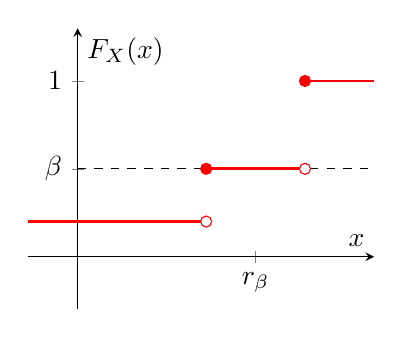
\begin{tikzpicture}
            \begin{axis}[
                xshift=170pt,
                width=170pt,
                ylabel=$F_X(x)$,
                xlabel=$x$,
                ymin=-0.3,ymax=1.3,
                xmin=-0.5,xmax=3,
                xtick = {1.8},
                xticklabels = {$r_\beta$},
                ytick = {0, 0.5, 1},
                yticklabels = {$0$, $\beta$, $1$},
            ] 
            \addplot[dashed, domain=0:3]{0.5};
            \addplot[cmhplot, domain=-0.5:1.3]{0.2};
            \addplot[cmhplot, domain=1.3:2.3]{0.5};
            \addplot[cmhplot, domain=2.3:3]{1};
            
            \addplot[holdot]coordinates{(1.3,0.2)(2.3,0.5)};
            \addplot[soldot]coordinates{(1.3,0.5)(2.3,1)};

                % \addplot[blue,smooth] {1/(1+exp(-x))};
            % \addlegendentry{Caso 2.}
            \end{axis}
            
        \end{tikzpicture}
    \end{center}
\end{figure}

Se invece la variabile $X$ ha densità, \emph{solitamente} esiste uno e un solo $\beta$-quantile, ed è il valore $r_\beta \in \R$ tale che $F_X(r_\beta) = \beta$.

\begin{example}
    Sia $X$ una variabile aleatoria con densità esponenziale, ovvero \[
        f(x) = \begin{cases}
            0, &\text{se } x \leq 0\\
            e^{-x}, &\text{se } x > 0.
        \end{cases}    
    \] La sua funzione di ripartizione è \[
        F_X(x) = \begin{cases}
            0, &\text{se } x \leq 0\\
            \int_0^x e^{-t}dt = 1 - e^{-x}, &\text{se } x > 0.
        \end{cases}    
    \] Il $\beta$-quantile di $X$ è quindi quel numero $r_\beta$ tale che \begin{align*}
        F_X(r_\beta) = 1 - e^{-r_\beta} = \beta \iff r_\beta = -\log\parens*{1 - \beta}.
    \end{align*} 
\end{example}

\section{Tipi più comuni di variabili aleatorie}
Definiamo ora i tipi più comuni di variabili aleatorie.

\subsection{Variabile binomiale}
La situazione concreta da cui nasce questa variabile aleatoria è ad esempio la seguente: vogliamo ripetere $n$ volte, in condizioni di indipendenza, un esperimento che può avere come risultato o il successo (con probabilità $p_0$), o l'insuccesso (con probabilità $1 - p_0$).
La variabile $X$ deve quindi contare il numero di successi in $n$ tentativi.

È chiaro quindi che i possibili valori che la variabile $X$ può assumere sono $0, 1, \dots, n$: negli $n$ tentativi posso avere $0$, $1$, $\dots$, oppure $n$ successi.

Calcoliamo ora la funzione di massa $p$: dato un qualsiasi $k \in \set{0, \dots, n}$ vogliamo calcolare la probabilità che la variabile aleatoria valga esattamente $k$, ovvero che su $n$ tentativi $k$ di essi siano successi.

La funzione di massa è la seguente: \[
    p(k) = \Prob\set[\big]{X = k} = \binom{n}{k}p_0^k(1-p_0)^{n-k}.
\] 
\begin{proof}
    Consideriamo una stringa di successi/insuccessi di lunghezza $n$. Esistono esattamente $\binom{n}{k}$ stringhe con $k$ successi; inoltre la probabilità ad essa associata è $p_0^k(1-p_0)^{n-k}$, in quanto ogni successo ha probabilità $p_0$ e ogni insuccesso ha probabilità $1-p_0$, da cui la tesi.
\end{proof}

Per esser certo che $p$ sia effettivamente una funzione di massa verifico che \[
    \sum_{k = 0}^n p(k) = 1.
\]
\begin{proof}
    Per definizione di $p$:
    \[
        \sum_{k = 0}^n p(k) = \sum_{k = 0}^n \binom{n}{k}p_0^k(1-p_0)^{n-k} = \parens[\Big]{p_0 + (1 - p_0)}^n = 1,
    \] dove il terzo passaggio è giustificato dal binomio di Newton.
\end{proof}

Se $n = 1$ la variabile $X$ viene detta \emph{di Bernoulli} di parametro $p_0$.

\subsection{Variabile geometrica}
Vogliamo ripetere, in condizioni di indipendenza, un esperimento che ha come risultati il successo (con probabilità $p_0$) oppure l'insuccesso (con probabilità $1 - p_0$) finché l'esperimento non ha successo. 

Come nel caso della variabile binomiale, la variabile aleatoria $X$ conta il numero di tentativi necessari: in questo caso però i valori possibili sono tutti i possibili valori naturali positivi insieme a $\set{+\infty}$, in quanto a priori il successo potrebbe non arrivare mai.

Calcoliamo ora la funzione di massa $p$: dato un qualsiasi $k \in \set{1, 2, \dots, +\infty}$ vogliamo calcolare la probabilità che la variabile aleatoria valga esattamente $k$, ovvero che i primi $k-1$ tentativi siano insuccessi e il $K$-esimo sia un successo. Nel caso $k = +\infty$, questo significa che tutti i tentativi sono insuccessi.

La funzione di massa legata a questa variabile è la seguente: \[
    p(k) = \Prob\set[\big]{X = k} = (1-p_0)^{k-1} \cdot p_0.
\]
\begin{proof}
    Siccome la probabilità di ogni insuccesso è di $1 - p_0$ e abbiamo $k-1$ insuccessi, la probabilità di ogni successo è $p_0$ e ne abbiamo uno solo, e gli eventi sono tutti indipendenti segue la tesi.
\end{proof}

Verifichiamo che $\sum p(k) = 1$:
\begin{align*}
    \sum_{k=1}^{+\infty} p(k) 
    &= \sum_{k=1}^{+\infty} \Prob{\set{X = k}}\\
    &= \sum_{k=1}^{+\infty} (1 - p_0)^{k-1} \cdot p\\
    &= p \cdot \sum_{k=1}^{+\infty} (1 - p_0)^{k-1}\\
    \intertext{Per ricondurmi alla serie geometrica pongo $h \deq k -1$, ottenendo}
    &= p \cdot \sum_{h=0}^{+\infty} (1 - p_0)^{h}\\
    &= p \cdot \frac{1}{1 - (1-p)}\\
    &= 1.
\end{align*}

La variabile geometrica ha un'altra interessante proprietà, detta \emph{proprietà dell'assenza di memoria}.
\begin{proposition}
    [Assenza di memoria della variabile geometrica]
    Siano $n, h \in \N$, $n, h > 0$ e sia $X$ una variabile aleatoria geometrica. Allora vale che \[
        \Prob[\Big]{\set[\big]{X = n + h} \given \set[\big]{X > n}} = \Prob\set[\big]{X = h}.    
    \]
\end{proposition}
\begin{proof}
    Per definizione di probabilità condizionata \begin{equation}
        \label{eq:tmp_abs_mem}
        \Prob[\Big]{\set[\big]{X = n + h} \given \set[\big]{X > n}}
        = \frac{\Prob\set[\big]{X = n + h}}{\Prob\set[\big]{X > n}}.
    \end{equation}
    Calcoliamo il denominatore di questa espressione: \begin{align*}
        \Prob\set[\big]{X > n}
        &= \sum_{h = n + 1}^\infty p(h)\\
        &= \sum_{h = n + 1}^\infty (1-p_0)^{h-1}\cdot p_0\\
        \intertext{Ponendo $k \deq h - n$, ovvero $h = k + n$:}
        &= \sum_{k = 1}^\infty (1-p_0)^{k+n-1} \cdot p_0\\
        &= (1 - p_0)^n \cdot \sum_{k = 1}^\infty (1-p_0)^{k-1}\cdot p_0\\
        &= (1 - p_0)^n,
    \end{align*}
    dove l'ultimo passaggio è giustificato dai calcoli fatti nel verificare la correttezza della funzione di massa della variabile binomiale.

    Sostituendo nella \eqref{eq:tmp_abs_mem}: \begin{align*}
        \frac{\Prob\set[\big]{X = n + h}}{\Prob\set[\big]{X > n}}
        &= \frac{(1+p_0)^{n+h-1} \cdot p_0}{(1-p_0)^n}\\
        &= (1-p_0)^{h-1}\cdot p_0\\
        &= \Prob\set[\big]{X = h}. \qedhere
    \end{align*}
\end{proof}

\subsection{Variabile di Poisson}
Si dice \emph{variabile di Poisson di parametro $\lambda$} (con $\lambda \in \R$, $\lambda > 0$) la variabile aleatoria con dominio $\N$ definita dalla seguente funzione di massa: \[
    p(h) = \Prob[\big]{\set{X = h}} \deq e^{-\lambda}\frac{\lambda^h}{h!}.    
\]
Verifichiamo che $\sum p(h) = 1$: \begin{align*}
    \sum_{h = 0}^\infty p(h)
    &= \sum_{h = 0}^\infty e^{-\lambda}\frac{\lambda^h}{h!}\\
    &= e^{-\lambda} \sum_{h = 0}^\infty \frac{\lambda^h}{h!}\\
    &= e^{-\lambda}e^{\lambda}\\
    &= 1.
\end{align*}

\subsection{Densità esponenziale}
Si definisce \emph{densità esponenziale di parametro $\lambda$} la funzione $f : \R \to \interval[{0, +\infty})$ tale che \[
    f(x) \deq \begin{cases}
        \lambda e^{-\lambda x}, &x \geq 0\\
        0, &x < 0.
    \end{cases} 
\]

Questa funzione è effettivamente una densità: infatti \begin{align*}
    \int_{-\infty}^{+\infty} f(x)dx
    &= \int_{-\infty}^0 0dx + \int_0^{+\infty} \lambda e^{-\lambda x}dx\\
    \intertext{Sostituendo $t \deq \lambda x$ (da cui $dt = \lambda dx$) l'integrale è equivalente a}
    &= \int_0^{+\infty} e^{-t}dt\\
    &= 1.
\end{align*}

La funzione di ripartizione corrispondente a questa densità è data da \begin{equation}
    \label{eq:cdf_exponential}
    F_X(x) = \int_{-\infty}^x f(t)dt = \begin{cases}
        0, &x < 0 \\[5pt]
        \displaystyle\int_0^x \lambda e^{-\lambda t}dt = 1 - e^{-\lambda x}, &x \geq 0.
    \end{cases}    
\end{equation}

La variabile esponenziale è \emph{senza memoria}, esattamente come la variabile binomiale, ovvero per ogni $s, t > 0$ vale che \[
    \Prob[\big]{\set{X \leq s + t} \given \set{X > s}} = \Prob[\big]{\set{X \leq t}}.    
\]
\begin{proof}
    Per definizione di probabilità condizionata:
    \begin{align*}
        \Prob[\big]{\set{X \geq s + t} \given \set{X > s}}
        &= \frac{\Prob[\big]{\set{X \leq s + t} \inters \set{X > s}}}{\Prob[\big]{\set{X > s}}}\\
        &= \frac{\Prob[\big]{\set{s < X \leq s + t}}}{\Prob[\big]{\set{X > s}}}.
    \end{align*}

    Facciamo alcune osservazioni generali:
    \begin{alignat*}{2}
        &(1):\; &&\Prob[\big]{\set{X > s}} = 1 - \Prob[\big]{\set{X \leq s}} = 1 - F_X(s).\\
        &(2):\; &&\begin{alignedat}[t]{1}
                \Prob[\big]{\set{s < X \leq s + t}} 
                &= \Prob[\big]{\set{X \leq s + t}} - \Prob[\big]{\set{X \leq s}} \\
                &= F_X(s+t) - F_X(s).
            \end{alignedat}
    \end{alignat*}

    Sostituendo nel nostro caso si ha \begin{align*}
        \frac{\Prob[\big]{\set{s < X \leq s + t}}}{\Prob[\big]{\set{X > s}}}
        &= \frac{F_X(s+t) - F_X(s)}{1 - F_X(s)}\\[3pt]
        &= \frac{1 - e^{-\lambda (s+t)} - (1 - e^{-\lambda s})}{1 - (1 - e^{-\lambda s})}\\[3pt]
        &= \frac{-e^{-\lambda s}e^{-\lambda t} + e^{-\lambda s}}{e^{-\lambda s}}\\[3pt]
        &= \frac{e^{-\lambda s}\parens*{1 - e^{-\lambda t}}}{e^{-\lambda s}}\\[3pt]
        &= 1 - e^{-\lambda t}\\[3pt]
        &= \Prob[\big]{X \leq t}. \qedhere
    \end{align*}
\end{proof}

\subsection{Variabile gaussiana}

Consideriamo la funzione $f(x) = e^{-\frac{x^2}{2}}$: anche se non ha una primitiva (esprimibile tramite funzioni elementari), si può calcolare il valore del suo integrale sulla retta reale, e si ha che \[
    \int_{\R} f(x) = \int_{-\infty}^{+\infty} e^{-\frac{x^2}{2}} = \sqrt{2\pi}.    
\] La conseguenza immediata di questo fatto è che dividendo la funzione per $\sqrt{2\pi}$ si ottiene una densità.

\begin{definition}
    [Densità Gaussiana standard] Si dice \emph{densità gaussiana standard} (o anche \emph{densità normale standard}) la funzione \[
        \phi(x) = \frac{1}{\sqrt{2\pi}}e^{\frac{x^2}{2}}.    
    \] La funzione di ripartizione ad essa associata è \[
        \Phi(x) = \frac{1}{\sqrt{2\pi}}\int_{\infty}^x e^{\frac{t^2}{2}}dt.
    \] La densità gaussiana standard si indica spesso con $\NormalDist*{0, 1}$; inoltre indicheremo con $q_\alpha$ lo $\alpha$-quantile della variabile $\NormalDist*{0, 1}$.
\end{definition}

\begin{remark}
    La densità $\phi$ è una funzione pari: infatti \[
        \phi(-x) = \frac{1}{\sqrt{2\pi}}e^{\frac{(-x)^2}{2}} =  \frac{1}{\sqrt{2\pi}}e^{\frac{x^2}{2}} = \phi(x).
    \]
\end{remark}

\begin{proposition}
    Vale la seguente proprietà per la funzione di ripartizione della $\NormalDist*{0, 1}$: \[
        \Phi(-x) = 1 - \Phi(x).    
    \]
\end{proposition}
\begin{proof} Siccome $\phi$ è pari:
    \begin{align*}
        \Phi(-x) &= \int_{-\infty}^{-x} \phi(t)dt \\
        &= \int_x^{+\infty} \phi(t)dt \\
        &= \int_x^{+\infty} \phi(t)dt + \int_{\infty}^{x} \phi(t)dt - \int_{\infty}^{x} \phi(t)dt\\
        &= \int_{-\infty}^{+\infty} \phi(t)dt - \int_{\infty}^{x} \phi(t)dt\\
        &= 1 - \Phi(x). \qedhere
    \end{align*}
\end{proof}
\begin{remark}
    Dalla proposizione precedente segue immediatamente che $\Phi(0) = \frac{1}{2}$.
\end{remark}

\begin{proposition}
    Vale la seguente proprietà per l'$\alpha$-quantile $q_\alpha$ della funzione di ripartizione della variabile gaussiana: \[
        q_{1-\alpha} = - q_{\alpha}.
    \]
\end{proposition}

La variabile $\NormalDist*{0, 1}$ può essere generalizzata (tramite una trasformazione) ad una variabile di parametri $m$ e $\sigma^2$, detta variabile $\NormalDist*{m, \sigma^2}$.

\begin{definition}
    [Variabile gaussiana $\NormalDist*{m, \sigma^2}$] Si dice variabile gaussiana $\NormalDist*{m, \sigma^2}$ la variabile $Y$ ottenuta a partire dalla variabile $X = \NormalDist*{0, 1}$ tramite la trasformazione \[
        Y = \sigma X + m.     
    \]
\end{definition}

Facciamo alcune osservazioni. \begin{itemize}
    \item La funzione di ripartizione di $Y$ è data da \[
        F_Y(y) = \Phi\parens*{\frac{y-m}{\sigma}}.    
    \] Infatti \begin{align*}
        F_Y(y) &= \Prob\set[\big]{Y \leq y} \\
        &= \Prob\set[\big]{\sigma X + m \leq y}\\
        &= \Prob\set[\Big]{X \leq \frac{y-m}{\sigma}}\\
        &= F_X\parens*{\frac{y-m}{\sigma}}\\
        &= \Phi\parens*{\frac{y-m}{\sigma}}.
    \end{align*}
    \item La densità di $Y$ è data da \[
        f_Y(y) = \frac{1}{\sigma\sqrt{2\pi}} e^{-\frac{(y-m)^2}{2\sigma^2}}.
    \] Infatti \begin{align*}
        f_Y(y) &= \frac{dF_Y(y)}{dy}\\
        &= \Phi^\prime\parens*{\frac{y-m}{\sigma}}\frac{1}{\sigma}\\
        &= \frac{1}{\sigma}\phi\parens*{\frac{y-m}{\sigma}}\\
        &= \frac{1}{\sigma\sqrt{2\pi}} e^{-\frac{(y-m)^2}{2\sigma^2}}.
    \end{align*}
\end{itemize}

Il principio fondamentale per descrivere le variabili gaussiane non standard è il seguente: se $Y$ è una variabile $\NormalDist*{m, \sigma^2}$, allora la variabile $\frac{Y-m}{\sigma}$ è standard.


\section{Trasformazioni di variabili aleatorie}

Consideriamo la variabile aleatoria $X$ con densità $f_X$: vogliamo studiare se, data una funzione $h$ qualsiasi, la variabile aleatoria definita da $Y \deq h \circ X$ è ancora con densità e in generale come fare per calcolarla.

In assenza di altre informazioni su $h$ l'unica strada è calcolare la funzione di ripartizione di $Y$: \[
    F_Y(y) = \Prob\set[\big]{Y \leq y} = \Prob\set[\big]{h \circ X \leq y}.    
\] Se essa è derivabile (o derivabile a tratti), derivandola in ogni punto in cui è possibile si ottiene la densità $f_Y$ di $Y$.

\begin{example}
    Consideriamo $X$ esponenziale di parametro $\lambda$ e la trasformazione $h : \R \to \R$ tale che $h(x) = x + 5$. Cerchiamo di vedere se la variabile $Y = h \circ X$ ha densità o meno: \begin{align*}
            F_Y(y) 
        &= \Prob\set[\big]{Y \leq y}\\
        &= \Prob\set[\big]{h \circ X \leq y} \\
        &= \Prob\set[\big]{X + 5 \leq y}\\
        &= \Prob\set[\big]{X \leq y - 5}\\
        &= F_X(y-5).
    \end{align*}

    Siccome abbiamo già calcolato la funzione di ripartizione della variabile esponenziale in \eqref{eq:cdf_exponential}, segue facilmente che la funzione di ripartizione di $Y$ è \[
        F_Y(y) = F_X(y-5) = \begin{cases}
            0, &y < 5\\
            1 - e^{-\lambda(y-5)}, &y \geq 5.
        \end{cases}    
    \] Derivando questa espressione si ha che la densità di $Y$ è \[
        f_Y(y) = \begin{cases}
            0, &y < 5\\
            \lambda e^{-\lambda(y-5)}, &y \geq 5,
        \end{cases}    
    \] ovvero la densità di $Y$ è la densità esponenziale traslata di $+5$.
\end{example}

Tuttavia in un caso particolare vi è una formula che ci permette di calcolare la densità senza passare per la funzione di ripartizione.

\begin{proposition} \label{prop:trasf_rand_var}
    Sia $X$ una variabile aleatoria la cui densità è non-nulla su un intervallo aperto $A \subseteq \R$. Sia $B \subseteq \R$ un altro intervallo aperto, $h : A \to B$ bigettiva e derivabile, con inversa derivabile. Allora $Y \deq h \circ X$ è una variabile aleatoria con densità data dalla formula \[
        f_Y(y) = \begin{cases}
            f_X\parens*{h\inv(y)} \abs*{\frac{dh\inv(y)}{dy}}, &y \in B\\
            0, &y \notin B.
        \end{cases}    
    \]
\end{proposition}

\begin{example}
    Consideriamo ancora una volta $X$ esponenziale di parametro $\lambda$ e la trasformazione $h : \R \to \R$ tale che $h(x) = x + 5$.

    Notiamo che la densità esponenziale è non-nulla nell'intervallo aperto $\interval[{0, +\infty})$ e la funzione $h$ è bigettiva, derivabile ed ha come inversa la funzione $h\inv(y) = y - 5$ che è a sua volta derivabile. 
    
    Per la \autoref{prop:trasf_rand_var} possiamo quindi trovare direttamente la densità di $Y$:
    se $y \in B = h\parens[\big]{\interval[{0, +\infty})} = \interval[{5, +\infty})$ vale che \begin{align*}
        f_Y(y) &= f_X\parens*{h\inv(y)} \abs*{\frac{dh\inv(y)}{dy}}\\
        &= f_X(y - 5) \abs*{\frac{d}{dy}(y - 5)}\\
        &= f_X(y-5)\\
        &= \lambda e^{-\lambda(y-5)}.
    \end{align*} Dunque la densità di $Y$ è data in generale da \[
        f_Y(y) = \begin{cases}
            0, &y < 5\\
            \lambda e^{-\lambda(y-5)}, &y \geq 5,
        \end{cases}
    \] che è lo stesso risultato ottenuto precedentemente.
\end{example}

\section{Variabili aleatorie doppie}

Una variabile aleatoria doppia è una funzione \[
    (X, Y) : \Omega \to \R^2    
\] a cui è associata una probabilità sui sottoinsiemi di $\R^2$: per ogni $A \subseteq \R^2$ deve essere definita \[
    \Prob_{X, Y}{A} = \Prob\set[\big]{(X, Y) \in A} = \Prob[\big]{(X, Y)\inv (A)}.   
\]
Come nel caso di una singola variabile aleatoria, possiamo avere variabili aleatorie doppie \emph{discrete} e \emph{con densità}.

\paragraph{Caso discreto} L'immagine della variabile aleatoria è un sottoinsieme finito o numerabile di $\R^2$. La funzione di massa sarà quindi \[
    p(x_i, y_i) = \Prob\set[\big]{X = x_i, Y = y_i},    
\] da cui per ogni insieme $A \subseteq \R^2$ la probabilità di $A$ è \[
    \Prob_{X, Y}{A} = \sum_{(x_i, y_i) \in A} p(x_i, y_i).    
\]

\paragraph{Caso con densità} In questo caso esiste una funzione $f : R^2 \to \interval[{0, +\infty})$ tale che \[
    \iint_{\R^2} f(x, y)dxdy = 1.    
\] La probabilità definita da questa densità è data da \[
    \Prob*_{X, Y}{A} = \iint_{A} f(x, y)dxdy    
\] per ogni $A \subseteq \R^2$.

\subsubsection{Leggi marginali}
Data una variabile aleatoria doppia $(X, Y)$ possiamo porci la domanda di ricavare le cosiddette \emph{leggi marginali}, ovvero le leggi di probabilità delle variabili $X$ e $Y$ prese separatamente.

\begin{proposition}
    Sia $(X, Y)$ una variabile aleatoria doppia.
    \begin{description}
        \item[Caso discreto] Se $(X, Y)$ è discreta con legge di massa $p_{X, Y}$, allora $X$ e $Y$ hanno rispettivamente funzioni di massa $p_X$ e $p_Y$ date da \[
            p_X(x_i) = \sum_{y_j}p_{X, Y}(x_i, y_j), \qquad  p_Y(y_j) = \sum_{x_i}p_{X, Y}(x_i, y_j).
        \]
        \item[Caso con densità] Se $(X, Y)$ è con densità e la sua densità è $f_{X, Y}$, allora $X$ e $Y$ hanno rispettivamente densità $f_X$ e $f_Y$ date da \[
            f_X(x) = \int_{\R}f_{X, Y}(x, y)dy, \qquad  f_Y(y) = \int_{\R}f_{X, Y}(x, y)dx.
        \]
    \end{description}
\end{proposition}
\begin{proof}
    Mostriamo solo il caso discreto. Notiamo che \[
        \set{X = x_i} = \bigdisjunion_{y_j} \set[\big]{X = x_i, Y = y_j},    
    \] da cui segue che \begin{align*}
        p_X(x_i) &= \Prob_{X}\set{X=x_i}\\
        &= \Prob*_{X}{\bigdisjunion_{y_j} \set[\big]{X = x_i, Y = y_j}}\\
        &= \sum_{y_j} \Prob_{X, Y}\set{X = x_i, Y = y_J}\\
        &= \sum_{y_j} p_{X, Y}(x_i, y_j). \qedhere
    \end{align*}
\end{proof}

Potremmo chiederci se sia possibile fare il contrario, ovvero trovare la legge della variabile $(X, Y)$ conoscendo le leggi marginali delle variabili $X$ e $Y$. La risposta è che ciò è impossibile, tranne nel caso in cui $X$ e $Y$ siano variabili \emph{indipendenti}.

\begin{definition}
    [Indipendenza di variabili aleatorie]
    Siano $X, Y : \Omega \to \R$ variabili aleatorie. $X$ e $Y$ si dicono \emph{indipendenti} se e solo se per ogni $A, B \in \R$ vale che gli eventi $X\inv(A)$ e $Y\inv(B)$ sono indipendenti, ovvero \[
        \Prob[\big]{X\inv(A) \inters Y\inv(B)} = \Prob[\big]{X\inv(A)}\Prob[\big]{Y\inv(B)},    
    \] o equivalentemente \[
        \Prob\set[\big]{X \in A, Y \in B} = \Prob\set[\big]{X \in A}\Prob\set[\big]{Y \in B}.     
    \]
\end{definition}

La prossima proposizione ci mostra una semplice caratterizzazione delle variabili indipendenti.
\begin{proposition}
    Siano $X, Y$ due variabili aleatorie. \begin{description}
        \item[Caso discreto] Se $X$ e $Y$ sono discrete, allora sono indipendenti se e solo se per ogni $x_i, y_j$ vale che \[
            p_{X, Y}(x_i, y_j) = p_X(x_i)p_Y(y_j).
        \]
        \item[Caso con densità] Se $X$ e $Y$ sono con densità, allora sono indipendenti se e solo se per ogni $x, y \in \R^2$ vale che \[
            f_{X, Y}(x, y) = f_X(x)f_Y(y).
        \]
    \end{description}
\end{proposition}
\begin{proof}
    Mostriamo soltanto il caso discreto: dimostriamo entrambi i versi dell'implicazione.
    \begin{description}
        \item[($\implies$)] Siano $x_i, y_j$ qualunque e siano $A = \set{x_i}$ e $B = \set{y_j}$. Allora \begin{align*}
            p(x_i, y_j) = \Prob\set[\big]{X = x_i, Y = y_j} = \Prob{X = x_i}\Prob{Y = y_j} = p_X(x_i)p_Y(y_j).
        \end{align*}
        \item[($\impliedby$)] Siano $A, B \subseteq \R$ qualunque. Allora \begin{align*}
            \Prob\set[\big]{X \in A, Y \in B} &= \sum_{x_i \in A, y_j \in B} p(x_i, y_j)\\
            &= \sum_{x_i \in A}\sum_{y_j \in B} p_X(x_i)p_Y(y_j)\\
            &= \parens*{\sum_{x_i \in A} p_X(x_i)} \parens*{\sum_{y_j \in B} p_Y(y_j)}\\
            &= \Prob\set[\big]{X \in A}\Prob\set[\big]{Y \in B},
        \end{align*} ovvero $X$ e $Y$ sono indipendenti. \qedhere
    \end{description}
\end{proof}

\subsection{Formule di convoluzione}

Consideriamo due variabili aleatorie $X$ e $Y$. La seguente formula ci permette di trovare la legge della variabile somma $X + Y$.

\begin{proposition}
    [Formule di convoluzione] Siano $X$, $Y$ due variabili aleatorie indipendenti. 
    \paragraph{Caso discreto} Se $X$, $Y$ sono discrete allora $Z \deq X + Y$ è una variabile aleatoria discreta la cui funzione di massa è \[
        p_Z(m) = \sum_{h = 0}^m p_X(h)p_Y(m-h).    
    \]
    \paragraph{Caso con densità} Se $X$, $Y$ sono con densità allora $Z \deq X + Y$ è una variabile aleatoria con densità la cui densità è \[
        f_Z(z) = \int_\R f_X(x)f_Y(z-x)dx = \int_\R f_X(z-y)f_Y(y)dy.
    \]
\end{proposition}

Le due formule precedenti, dette rispettivamente \emph{formula di convoluzione discreta} e \emph{fomula di convoluzione}, sono utilissime per descrivere le somme di variabili aleatorie.

\begin{proof}
    Dimostriamo la formula di convoluzione discreta. Essa deriva direttamente dall'uguaglianza insiemistica \[
        \set{X+Y = m} = \bigdisjunion_{h = 0}^m \set{X = h, Y = m-h};    
    \] siccome i due insiemi sono uguali anche le loro probabilità lo saranno, da cui la tesi.
\end{proof}
\section{Valore atteso e momenti}

Nel primo capitolo abbiamo introdotto il concetto di media empirica: data una collezione di dati $\vec x = (x_1, \dots, x_n)$ possiamo calcolarne il valore medio con la formula \[
    \frac1n \sum_{i = 1}^n x_i. 
\] Potremmo generalizzare questa formula come la somma pesata dei valori assunti da una variabile aleatoria $X$, ognuno moltiplicato per il valore della funzione di massa in quel punto: \[
    \sum_{x_i} x_i p(x_i). 
\] Tuttavia nel caso di variabili che prendono infiniti valori dobbiamo prima assicurarci che la serie converga. Diamo quindi la seguente definizione.

\begin{definition}
    [Valore atteso] Sia $X$ una variabile aleatoria.
    \paragraph{Caso discreto} Se $X$ è discreta e vale che \[
        \sum_{x_i} \abs{x_i}p(x_i) < +\infty
    \] si dice che $X$ ha \emph{valore atteso} (oppure \emph{speranza matematica}, oppure ancora \emph{momento primo}) e il valore atteso di $X$ è \[
        \Expect{X} = \sum_{x_i} x_ip(x_i).    
    \]
    \paragraph{Caso discreto} Se $X$ è con densità e vale che \[
        \int_\R \abs{x}f_X(x)dx < +\infty
    \] si dice che $X$ ha \emph{valore atteso} e il valore atteso di $X$ è \[
        \Expect{X} = \int_\R xf_X(x)dx.    
    \]
\end{definition}

\begin{remark}
    Osserviamo che siccome la funzione di massa di una variabile aleatoria è sempre non-negativa, allora \[
        \Expect[\big]{\abs{X}} = \sum_{x_i} \abs*{x_ip(x_i)} = \sum_{x_i} \abs*{x_i}p(x_i).   
    \] Segue quindi che $X$ ha momento primo se e solo se $\Expect[\big]{\abs{X}} < +\infty$. Un risultato analogo ovviamente vale per le variabili con densità.
\end{remark}
\section{Funzione generatrice dei momenti}

Data una variabile aleatoria $X$ possiamo considerare la variabile aleatoria derivata $e^{tX}$: essa è sempre maggiore o uguale di $0$, dunque ha sicuramente senso calcolarne il valore atteso (che quindi è un numero reale positivo oppure più infinito).

\begin{definition}
    [Funzione generatrice dei momenti]
    Si dice \strong{funzione generatrice dei momenti} della variabile aleatoria $X$ la funzione \[
        G_X(t) \deq \Expect[\big]{e^{tX}} = \begin{cases}
            \displaystyle \sum_{x_i} e^{tx_i}p(x_i), &X \text{ discreta},\\
            \displaystyle \int_\R e^{tx}f(x), &X \text{ con densità}.
        \end{cases}
    \] Si chiama \strong{dominio} di $G_X$ l'insieme dei $t \in \R$ tali che $G_X(t) < +\infty$.
\end{definition}

Osserviamo che $0$ appartiene necessariamente al dominio di $G_X$, in quanto \[
    G_X(0) = \Expect[\big]{e^{0X}} = \Expect{1} = 1. 
\] Segue quindi che il dominio della funzione generatrice è il singolo punto $t = 0$ oppure contiene almeno un intervallo $\interval({-\eps, \eps})$ centrato in $0$.

\begin{theorem}
    Siano $X$, $Y$ due variabili aleatorie tali che i domini di $G_X$ e $G_Y$ contengano entrambe un intervallo aperto $\interval({-\eps, \eps})$ e che si abbia $G_X(t) = G_Y(t)$ per ogni $t \in \interval({-\eps, \eps})$. Allora $X$ e $Y$ sono equidistribuite, ovvero hanno la stessa distribuzione di probabilità.
\end{theorem}

\begin{proposition}
    [Proprietà della funzione generatrice]
    Sia $X$ una variabile aleatoria.
    \begin{enumerate}[label={(\roman*)}]
        \item Se $Y \deq aX + B$, allora \[
            G_Y(t) = e^{tb} G_X(at).
        \]
        \item Se $Z$ è una variabile aleatoria e $X$, $Z$ sono indipendenti, allora \[
            G_{X + Z}(t) = G_X(t)G_Z(t).    
        \]
    \end{enumerate}
\end{proposition}
\begin{proof}
    La dimostrazione della prima proprietà è immediata: \begin{align*}
        G_Y(t)
        = \Expect*{e^{(aX + b)t}}
        = \Expect*{e^{atX}e^{bt}}
        = e^{bt}\Expect*{e^{atX}}
        = e^{bt}G_X(at).
    \end{align*}
    Per la seconda, basta osservare che $e^{tX}$ e $e^{tZ}$ sono indipendenti, dunque per la \autoref{prop:prop_expect} (in particolare per il terzo punto) vale che \begin{align*}
        G_{X + Z}(t)
        = \Expect*{e^{(X + Z)t}}
        = \Expect*{e^{tX}e^{tZ}}
        = \Expect*{e^{tX}}\Expect*{e^{tZ}}
        = G_X(t)G_Z(t).
    \end{align*}
\end{proof}

Il motivo per cui la funzione generatrice dei momenti ha questo nome deriva dal prossimo risultato: in alcuni casi possiamo usarla per calcolare i momenti di una variabile aleatoria.

\begin{theorem}
    [Generazione dei momenti] Sia $X$ una variabile aleatoria tale che esista un intervallo $\interval({-\eps, \eps})$ completamente contenuto nel dominio di $G_X$. Allora $X$ possiede tutti i momenti e vale che \[
        \Expect[\big]{X^n} = G_X^{(n)}(0),    
    \] dove $G_X^{(n)}$ è la derivata $n$-esima di $G_X$.
\end{theorem}

Possiamo dare una dimostrazione intuitiva del teorema nel caso di $n = 1$ nel seguente modo: \[
    G_X^\prime(t) = \frac{d}{dt}\Expect[\big]{e^{tX}} = 
    \Expect*{\frac{d}{dt}e^{tX}} = \Expect[\big]{Xe^{tX}},
\] dunque per $t = 0$ si ha esattamente $G_X^\prime(t) = \Expect[\big]{X}$.

\subsection*{Esempi}

% TODO

\section{Teoremi limite}

In questa sezione considereremo il comportamento al limite di una successione $\seqn{X_n}$ di variabili aleatorie indipendenti ed equidistribuite. Enunciamo i due teoremi limite fondamentali.

\begin{theorem}
    [Legge Debole dei Grandi Numeri]
    \label{th:law_large_numbers}
    Sia $\seqn{X_n}$ una successione di variabili aleatorie indipendenti ed equidistribuite, dotate tutte di momento secondo. Sia inoltre $\mu \deq \Expect[\big]{X_i}$ il loro valore atteso.

    Allora per ogni $\eps > 0$ vale che \begin{equation}
        \lim_{n \to +\infty} \Prob*{\abs*{\frac{X_1 + \dots + X_n}{n} - \mu} > \eps} = 0.    
    \end{equation}
\end{theorem}

\begin{theorem}
    [Teorema del Limite Centrale]
    \label{th:central_limit}
    Sia $\seqn{X_n}$ una successione di variabili aleatorie indipendenti ed equidistribuite. Sia inoltre $\mu \deq \Expect[\big]{X_i}$ il loro valore atteso e $\sigma^2 \deq \Var{X_i}$ la loro varianza.

    Allora per ogni $\infty \leq a < b \leq +\infty$ vale che \begin{equation}
        \lim_{n \to +\infty} \Prob*{a \leq \frac{X_1 + \dots + X_n - n\mu}{\sigma\sqrt{n}} \leq b} = \Phi(b) - \Phi(a),  
    \end{equation}
    dove $\Phi$ è la funzione di ripartizione dela variabile aleatoria gaussiana standard.
\end{theorem}

Iniziamo studiando la \nameref{th:law_large_numbers} con una definizione.
\begin{definition}
    [Convergenza in probabilità]
    Sia $\seqn{X_n}$ una successione di variabili aleatorie. Si dice che $\seqn{X_n}$ \strong{converge in probabilità} alla variabile aleatoria $X$ se per ogni $\eps > 0$ si ha \[
        \lim_{n \to +\infty} \Prob[\big]{\abs{X_n - X} > \eps} = 0.    
    \]
\end{definition}

Diamo una semplice condizione sufficiente per la convergenza in probabilità.
\begin{proposition}
    [Condizione sufficiente per la convergenza in probabilità]
    \label{prop:cond_suff_conv_prob} Sia $\seqn{X_n}$ una successione di variabili aleatorie tale che \[
        \lim_{n \to +\infty} \Expect[\big]{X_n} = c \in \R, \qquad \lim_{n \to +\infty} \Var{X_n} = 0.    
    \] Allora $\seqn{X_n}$ converge in probabilità alla costante $c$.
\end{proposition}
\begin{proof}
    Sia $\eps > 0$ qualunque. Per la \nameref{prop:dis_Markov} sostituendo $Y = (X_n - c)^2$, $a \deq \eps^2$ si ha \[
        \eps^2\Prob[\big]{(X_n - c)^2 > \eps^2} = \eps^2\Prob[\big]{\abs{X_n - c} > \eps} \leq \Expect[\big]{(X_n - c)^2},
    \] ovvero \begin{equation}
        \Prob[\big]{\abs{X_n - c} > \eps} \leq \frac{\Expect[\big]{(X_n - c)^2}}{\eps^2}. \label{eq:dis_cond_suff_conv_prob}
    \end{equation} Tuttavia \begin{align*}
        &\Expect[\big]{(X_n - c)^2}\\
        = {}&\Expect[\Big]{\parens[\big]{X_n - \Expect{X_n} + \Expect{X_n} - c}^2}\\
        = {}&\Expect[\Big]{\parens[\big]{X_n - \Expect{X_n}}^2 + \Expect[\big]{2(X_n - \Expect{X_n})(\Expect{X_n} - c)} + \parens[\big]{\Expect{X_n} - c}^2}\\
        = {}&\Expect[\Big]{\parens[\big]{X_n - \Expect{X_n}}^2} + 2(\Expect{X_n} - c)\Expect[\big]{X_n - \Expect{X_n}} + \parens[\big]{\Expect{X_n} - c}^2\\
        = {}&\Var{X_n} + \parens[\big]{\Expect{X_n} - c}^2.
    \end{align*}
    Di conseguenza $\Expect[\big]{(X_n - c)^2} \to 0$, dunque per la disuguaglianza \eqref{eq:dis_cond_suff_conv_prob} segue che \[
        \Prob[\big]{\abs{X_n - c} > \eps} \to 0,
    \] ovvero la successione $\seqn{X_n}$ converge in probabilità a $c$.
\end{proof}

Possiamo quindi dimostrare la \nameref{th:law_big_numbers}.
\begin{proof}
    [Dimostrazione della \nameref{th:law_large_numbers}]
    Sia $\bar X_n$ la variabile aleatoria definita da: \[
        \bar X_n \deq \frac{1}{n}\sum_{i = 1}^{n}X_i = \frac{X_1 + \dots + X_n}{n}.
    \] Allora si ha che il valore atteso di $\bar X_n$ è \[
       \Expect[\big]{\bar X_n} = \frac{\Expect[\big]{X_1} + \dots + \Expect[\big]{X_n}}{n} = \frac{n\mu}{n} = \mu, 
    \] mentre la sua varianza è \begin{align*}
        \Var{\bar X_n} 
        &= \Var*{\frac1n \sum_{i = i}^n X_i} \\
        &= \frac{1}{n^2} \sum_{i = 1}^n \Var{X_i}\\
        &= \frac{n\sigma^2}{n^2}\\
        &= \frac{\sigma^2}{n} \xrightarrow{n \to +\infty} 0.
    \end{align*} Per la \autoref{prop:cond_suff_conv_prob} segue quindi che $\seqn*{\bar X_n}$ converge in probabilità a $\mu$, ovvero \[
        \lim_{n \to +\infty} \Prob*{\abs*{\bar X_n - \mu} > \eps} = 0. \qedhere
    \]
\end{proof}

In realtà le ipotesi del teorema possono essere indebolite: è sufficiente che 
\begin{itemize}
    \item le variabili $X_i$ siano \emph{incorrelate} (non è necessario che siano indipendenti);
    \item le variabili abbiano tutte lo stesso valore atteso $\mu$;
    \item le varianze siano \emph{equilimitate} (invece di essere tutte uguali a $\sigma^2$), ovvero che esista $M \in \R$ tale che $\Var{X_i} \leq M$ per ogni $i$.
\end{itemize}

Per quanto riguarda il \nameref{th:central_limit}, esso afferma che, per $n$ \emph{sufficientemente grande}, la variabile \[
    \frac{X_1 + \dots + X_n - n\mu}{\sigma\sqrt{n}} = \sqrt{n} \frac{\bar X_n - n\mu}{\sigma}    
\] è approssimativamente una Gaussiana standard. Questa approssimazione comincia a diventare sufficientemente precisa per $n \geq 80$, e viene usata soprattutto per approssimare variabili binomiali di parametri $n$ e $p$: infatti siccome una binomiale $X \sim B(n, p)$ del genere è uguale alla somma di $n$ variabili di Bernoulli, segue che la variabile \[
    \frac{X - np}{\sqrt{np(1-p)}}
\] è approssimativamente $N(0, 1)$.
\section{Altre densità importanti}

\subsection{Densità gamma}

Definiamo innanzitutto la funzione Gamma di Eulero come \[
    \Gamma(r) \deq \int_0^{+\infty} x^{r-1}e^{-x} dx.   
\] Anche se questo integrale non è calcolabile direttamente, per $r > 1$ vale la relazione \[
    \Gamma(r) = (r-1)\Gamma(r-1).
\] Infatti integrando per parti si ha \begin{align*}
    \Gamma(r) &= \int_0^{+\infty} x^{r-1}e^{-x} dx\\
    &= \EvaluateAt[\bigg]{-x^{r-1}e^{-x}}_0^{+\infty} + (r-1)\int_0^{+\infty} x^{r-2}e^{-x} dx\\
    &= (r-1)\Gamma(r-1).
\end{align*} Inoltre siccome $\Gamma(1) = 1$ si ha che $\Gamma(n) = (n-1)!$ per ogni $n \in \N \setminus \set{0}$.

Definiamo quindi la densità gamma.
\begin{definition}
    [Densità gamma] Siano $r, \lambda > 0$. Si dice \strong{densità gamma di parametri $r$ e $\lambda$} la densità data da \[
        f(x) \deq \begin{cases}
            \displaystyle \frac{1}{\Gamma(r)}\lambda^r x^{r-1} e^{-\lambda x}, &x > 0\\[2pt]
            0,                                                         &x \leq 0.
        \end{cases}    
    \]
\end{definition}
Questa funzione è effettivamente una densità: infatti \begin{align*}
    \int_0^{+\infty} \frac{1}{\Gamma(r)}\lambda^r x^{r-1} e^{-\lambda x} dx
    &= \frac{1}{\Gamma(r)} \int_0^{+\infty} (x\lambda)^{r-1} e^{-\lambda x} \lambda dx\\[2pt]
    &= \frac{1}{\Gamma(r)} \int_0^{+\infty} t^{r-1} e^{-t}dt\\[2pt]
    &= \frac{1}{\Gamma(r)} \cdot \Gamma(r)\\
    &= 1.
\end{align*}

\begin{remark}
    La densità esponenziale di parametro $\lambda$ è semplicemente una densità $\Gamma(1, \lambda)$.
\end{remark}

\begin{proposition}
    [Momenti della densità gamma]
    Sia $X$ una variabile aleatoria di densità $\Gamma(r, \lambda)$. Allora $X$ possiede tutti i momenti e preso $\beta \in \R, \beta > 0$ si ha che \[
        \Expect[\big]{X^\beta} = \frac{\Gamma(r+\beta)}{\Gamma(r)\lambda^\beta}.    
    \] 
\end{proposition}
\begin{proof}
    Siccome $X$ prende solo valori positivi, possiamo scrivere \begin{align*}
        \Expect[\big]{X^\beta} &=  \frac{1}{\Gamma(r)} \int_0^{+\infty} x^\beta \lambda^r x^{r-1} e^{-\lambda x} dx.\\
        \intertext{Moltiplicando e dividendo per $\lambda^\beta$ si ha che}
        &= \frac{1}{\Gamma(r)\lambda^\beta} \int_0^{+\infty} \lambda^{r+\beta} x^{\beta+r-1} e^{-\lambda x} dx\\[2pt]
        &= \frac{\Gamma(r+\beta)}{\Gamma(r)\lambda^\beta}. \qedhere
    \end{align*}
\end{proof}

Da questa proposizione riusciamo a calcolare semplicemente tutti i momenti: infatti ad esempio \[
    \Expect[\big]{X} = \frac{\Gamma(r+1)}{\Gamma(r)\lambda} = \frac{r\Gamma(r)}{\Gamma(r)\lambda} = \frac{r}{\lambda},    
\] oppure anche \[
    \Expect[\big]{X^2} = \frac{\Gamma(r+2)}{\Gamma(r)\lambda^2} = \frac{r(r+1)}{\lambda^2},    
\] da cui $\Var{X} = \dfrac{r}{\lambda^2}$.

\begin{proposition}
    [Funzione generatrice della densità gamma]
    Sia $X$ una variabile aleatoria con densità $\Gamma(r, \lambda)$. Allora $G_X(t)$ è finito se e solo se $t < \lambda$ e in tal caso si ha \[
        G_X(t) = \parens*{\frac{\lambda}{\lambda - t}}^r.    
    \]
\end{proposition}
\begin{proof}
    Dalla definizione di funzione generatrice dei momenti si ha \begin{align*}
        \Expect*{e^{tX}} 
        &= \frac{1}{\Gamma(r)}\int_0^{+\infty} e^{tx} \lambda^r x^{r-1} e^{-\lambda x} dx.\\
        \intertext{Moltiplicando e dividendo per $(\lambda - t)^r$ si ha}
        &= \frac{\lambda^r}{\Gamma(r)(\lambda - t)^r} \int_0^{+\infty}  (\lambda - t)^r x^{r-1} e^{-(\lambda - t)x} dx\\[3pt]
        &= \frac{\lambda^r}{\Gamma(r)(\lambda - t)^r} \Gamma(r)\\[3pt]
        &= \parens*{\frac{\lambda}{\lambda - t}}^r. \qedhere
    \end{align*}
\end{proof}

Come conseguenza immediata se $X \sim \Gamma(r, \lambda)$ e $Y \sim \Gamma(s, \lambda)$ e $X, Y$ sono indipendenti, allora $X + Y \sim \Gamma(r + s, \lambda)$.

\subsection{Densità chi-quadro}

\begin{definition}
    [Densità chi-quadro]
    Siano $X_1, \dots, X_n$ variabili gaussiane standard indipendenti. La densità della variabile \[
        C_n \deq X_1^2 + \dots + X_n^2    
    \] si chiama \strong{densità chi-quadro ad $n$ gradi di libertà}, e la si indica con $\chi^2(n)$.
\end{definition}

\begin{proposition}
    La densità $\chi^2(n)$ è uguale alla densità $\Gamma(\nicefrac{n}{2}, \nicefrac{1}{2})$.
\end{proposition}
\begin{proof}
    È sufficiente dimostrare che se $X$ è gaussiana standard allora $X^2$ ha densità $\Gamma(\nicefrac{1}{2}, \nicefrac{1}{2})$.

    Consideriamo la funzione generatrice di $X^2$. Essa è uguale a \begin{align*}
        G_{X^2}(t) &= \Expect*{e^{tX^2}}\\[3pt]
        &= \frac{1}{\sqrt{2\pi}} \int_{\R} e^{tx^2}e^{-\frac{x^2}{2}} dx\\[3pt]
        &= \frac{1}{\sqrt{2\pi}} \int_{\R} e^{-\frac{x^2}{2}(1 - 2t)} dx.\\[3pt]
        \intertext{Siccome $\int_{\R} e^{-\frac{x^2}{2\sigma^2}} = \sqrt{2\pi} \cdot \sigma$, ponendo $\sigma \deq \parens*{1 - 2t}^{-\nicefrac12}$ si ottiene }
        &= \frac{1}{\sqrt{2\pi}} \sqrt{\frac{2\pi}{1-2t}}\\[3pt]
        &= \sqrt{\frac{1}{1-2t}}\\[3pt]
        &= \parens*{\frac{\nicefrac12}{\nicefrac12 - t}}^\frac12,
    \end{align*} che è proprio la funzione generatrice della funzione $\Gamma(\nicefrac{1}{2}, \nicefrac12)$.
\end{proof}

Lo $\alpha$-quantile della variabile $\chi^2(n)$ è denotato con $\chi^2_{(\alpha, n)}$.

Osserviamo che non è necessario calcolare nuovamente i momenti o la funzione generatrice di questa variabile, in quanto essa si comporta esattamente come una variabile $\Gamma(\nicefrac{n}{2}, \nicefrac12)$; in particolare la somma di due variabili indipendenti $X \sim \chi^2(n)$, $Y \sim \chi^2(m)$ è una variabile $(X + Y) \sim \chi^2(n + m)$.

Inoltre se $C_n$ ha densità $\chi^2(n)$, allora possiamo pensarla come somma di $n$ quadrati di variabili gaussiane $X_i$: per quanto abbiamo visto sulle variabili gaussiane vale che \[
    \Expect[\big]{X_i^2} = 1, \qquad \Var*{X_i^2} = 2.    
\] Valgono quindi i seguenti due risultati: \begin{itemize}
    \item per la \nameref{th:law_large_numbers} vale che $\dfrac{C_n}{n} \approx 1$ per $n \to +\infty$;
    \item per il \nameref{th:central_limit} vale che la successione $\seqn*{\dfrac{C_n - n}{\sqrt{2n}}}$ converge in distribuzione ad una variabile gaussiana standard, e quindi per $n$ sufficientemente grande la variabile $\dfrac{C_n - n}{\sqrt{2n}}$ è approssimativamente una gaussiana standard.
\end{itemize}

\subsection{Densità di Student}

\begin{definition}
    [Densità di Student] Sia $X \sim \NormalDist*{0, 1}$, $C_n \sim \chi^2(n)$ e siano le due indipendenti. La densità della variabile \[
        T_n \deq \frac{X}{\sqrt{\frac{C_n}{n}}} = \sqrt n \frac{X}{\sqrt{C_n}} 
    \] si dice \strong{densità di Student a $n$ gradi di libertà}.
\end{definition}

Osserviamo che una variabile di Student è pari, in quanto la variabile gaussiana è pari: da questo segue che la densità di Student è pari e valgono relazioni simili a quelle descritte per la funzione di ripartizione e per i quantili della variabile gaussiana. In particolare se $F_n$ è la funzione di ripartizione di una variabile di Student con $n$ gradi di libertà vale che \[
    F_n(-x) = 1 - F_n(x),    
\] mentre se $\tau_{(\alpha, n)}$ è l'$\alpha$-quantile di una variabile di Student ad $n$ gradi di libertà vale che \[
    \tau_{(\alpha, n)} = -\tau_{(1-\alpha, n)}.
\]

Inoltre per definizione quando $n$ è sufficientemente grande una variabile di Student a $n$ gradi di libertà può essere approssimata con una variabile gaussiana: infatti siccome $\frac{C_n}{n} \approx 1$ quando $n$ è grande segue che \[
    T_n = \frac{X}{\sqrt{\frac{C_n}{n}}} \approx \frac{X}{1} = X.    
\]

\chapter{Inferenza statistica}
\section{Primi cenni di inferenza statistica}

Lo scopo dell'inferenza statistica è quello di partire da un certo campione, analizzarne i dati e dedurre informazioni sull'intera popolazione. Per fare ciò si suppone che vi sia un'implicita distribuzione di probabilità nell'intera popolazione e che le osservazioni del campione siano le realizzazioni di un insieme di variabili aleatorie indipendenti aventi questa distribuzione di probabilità.

\begin{definition}
    [Campione statistico] Si dice \strong{campione statistico} o \strong{aleatorio} una famiglia di $n$ variabili aleatorie indipendenti $X_1, \dots, X_n$ con la stessa funzione di ripartizione $F$.
\end{definition}

Diremo che $n$ è la \emph{taglia} del campione mentre la funzione di ripartizione $F$ sarà chiamata \emph{legge di probabilità} del campione.

\begin{definition}
    [Statistica campionaria] Una funzione $g(X_1, \dots, X_n)$ di un campione viene detta \strong{statistica campionaria}.
\end{definition}

Esempi di statistiche campionarie sono la \emph{media campionaria} e la \emph{varianza campionaria}, definite rispettivamente da \begin{align*}
    \bar X \deq \frac{X_1 + \dots + X_n}{n},\\[3pt]
    S^2 \deq \frac{\displaystyle \sum_{i = 1}^n \parens*{X_i - \bar X}}{n-1}.
\end{align*}
Una statistica campionaria viene detta \strong{stima corretta} se il suo valore atteso conincide con la quantità che si vuole stimare. Mostriamo che la media campionaria e la varianza campionaria sono stime corrette rispettivamente del valore atteso e della varianza delle variabili del campione.

\begin{proposition}
    [Correttezza delle stime della media e varianza campionaria]
    Sia $X_1, \dots, X_n$ un campione statistico. Supponiamo che le variabili ammettano momento secondo e siano $\mu = \Expect[\big]{X_i}$ e $\sigma^2 = \Var[\big]{X_i}$. Allora si ha che \[
        \Expect[\Big]{\bar X} = \mu, \qquad \Expect*{\frac{\sum_{i = 1}^n \parens[\big]{X_i^2 - \bar X}}{n - 1}} = \sigma^2.
    \]
\end{proposition}
\begin{proof}
    Innanzitutto ricordiamo che vale l'uguaglianza \[
        \sum_{i = 1}^n \parens[\big]{X_i - \bar X}^2 = \parens*{\sum_{i = 1}^n X_i^2} - n\bar X^2.    
    \]
    \begin{itemize}
        \item Per quanto riguarda il valore atteso di $\bar X$ si ha che \[
            \Expect[\Big]{\bar X} 
            = \Expect*{\frac{X_1 + \dots X_n}{n}} 
            = \frac1n\parens[\Big]{\Expect[\big]{X_1} + \dots \Expect[\big]{X_n}}     
            = \frac{n\mu}{n} = \mu.
        \]
        \item Osserviamo che la varianza di $\bar X$ è data da \[
            \Expect[\Big]{\bar X} 
            = \Var*{\frac{X_1 + \dots X_n}{n}} 
            = \frac1{n^2}\parens[\Big]{\Var[\big]{X_1} + \dots + \Var[\big]{X_n}}     
            = \frac{n\sigma^2}{n^2} = \frac{\sigma^2}{n}.  
        \] Da ciò segue che \[
            \Expect[\Big]{\bar X^2} = \Expect[\Big]{\bar X}^2 + \Var[\Big]{\bar X} = \mu^2 + \frac{\sigma^2}{n}.
        \] Inoltre \[
            \Expect[\Big]{X_i^2} = \Expect[\big]{X_i}^2 + \Var[\big]{X_i} = \mu^2 + \sigma^2.    
        \] Quindi vale che \begin{align*}
            \Expect*{\sum_{i = 1}^n \parens[\big]{X_i^2 - \bar X}}
            &= \parens*{\sum_{i = 1}^n \Expect*{X_i^2}} - n\Expect[\Big]{\bar X^2}\\
            &= n\parens*{\sigma^2 + \mu^2} - n\parens*{\frac{\sigma^2}{n} + \mu^2}\\
            &= (n-1)\sigma^2,
        \end{align*}
        che è la tesi. \qedhere
    \end{itemize}
\end{proof}

\section{Stime parametriche}

In alcuni casi la distribuzione di probabilità nascosta che si vuole studiare è parzialmente specificata, nel senso che sappiamo che appartiene ad una famiglia di funzioni di ripartizione dipendenti da un opportuno parametro, usualmente indicato con $\theta$, che è incognito.

Supponiamo quindi di avere un campione statistico la cui legge di probabilità dipende da un parametro $\theta \in \Theta$.
\begin{definition}
    [Verosimiglianza] Si dice \strong{verosimiglianza} del campione $X_1, \dots, X_n$ la funzione $L(\theta, x_1, \dots, x_n)$ definita da \[
        L(\theta, x_1, \dots, x_n) = \begin{cases}
            \displaystyle \prod_{i = 1}^n p_\theta(x_i), &\text{se le variabili sono discrete},\\[7pt]
            \displaystyle \prod_{i = 1}^n f_\theta(x_i), &\text{se le variabili sono con densità.}\\[5pt]
        \end{cases}  
    \]
\end{definition}

\begin{definition}
    [Stima di massima verosimiglianza] Sia $X_1, \dots, X_n$ un campione statistico la cui legge di probabilità dipende dal parametro $\theta \in \Theta$. Se esiste un valore $\hat\theta \in \Theta$ tale che \[
        L\parens*{\hat\theta, x_1, \dots, x_n} = \max_{\theta \in \Theta} L(\theta, x_1, \dots, x_n),
    \] esso si dice \strong{stima di massima verosimiglianza} del campione $X_1, \dots, X_n$.
\end{definition}

Un altro metodo di stima è la \strong{stima col metodo dei momenti}: l'idea è di uguagliare i momenti teorici con i momenti empirici per ricavare il valore di $\theta$, o più in generale dei parametri $\theta_1, \dots, \theta_h$. Calcoliamo quindi i momenti teorici mediante il modello: \[
    \Expect*_{\theta_1, \dots, \theta_h}{X^k}        
\] e li confrontiamo con i momenti empirici: \[
    \sum_{i=1}^n \frac{x_i^k}{n}.    
\] 

Se esiste una scelta di $\theta_1, \dots, \theta_n$ tale che \[
    \Expect*_{\theta_1, \dots, \theta_h}{X^k} = \sum_{i=1}^n \frac{x_i^k}{n}
\] allora abbiamo stimato la legge di probabilità del campione tramite il metodo dei momenti. Useremo la notazione $\tilde\theta$ per indicare la stima di $\theta$ con il metodo dei momenti.

\begin{example}
    Supponiamo di avere un campione statistico di $n$ variabili con densità esponenziale di parametro $0 < \theta < +\infty$. Supponiamo inoltre di avere un campione di osservazioni $x_1, \dots, x_n$ \emph{positive}.

    Siccome $\Expect_{\theta}[\big]{X_i} = \nicefrac{1}{\theta}$, la stima col metodo dei momenti si ottiene uguagliando \[
        \sum_{i=1}^n \frac{x_i}{n} = \frac{1}{\theta} \;\implies\; \tilde\theta = \frac{1}{\bar x}.     
    \]

    Allo stesso modo la funzione di verosimiglianza è data da \[
        L(\theta, x_1, \dots, x_n) = \prod_{i=1}^n f_\theta(x_i) = \prod_{i=1}^n \theta e^{-\theta x_i} = \theta^n e^{-\theta \sum_{i=1}^n x_i}.
    \] Osserviamo che questa funzione tende a $0$ per $x \to 0$, $x \to +\infty$: siccome è una funzione positiva segue che ha massimo. La sua derivata rispetto a $\theta$ è \[
        L'(\theta, x_1, \dots, x_n) = n\theta^{n-1}e^{-\theta\sum_{i=1}^n x_i} - \theta^n e^{-\theta\sum_{i=1}^n x_i} \cdot \parens*{\sum_{i=1}^n x_i};
    \] ponendola uguale a $0$ otteniamo \begin{align*}
        &n\theta^{n-1}e^{-\theta\sum_{i=1}^n x_i} - \theta^n e^{-\theta\sum_{i=1}^n x_i} \cdot \parens*{\sum_{i=1}^n x_i} = 0\\
        \iff {}&\theta^{n-1}e^{-\theta\sum_{i=1}^n x_i} \cdot \parens*{n - \theta \cdot \parens*{\sum_{i=1}^n x_i}} = 0\\
        \iff {}&n - \theta \cdot \parens*{\sum_{i=1}^n x_i} = 0\\
        \iff {}&\theta = \frac{n}{\sum_{i=1} x_i} = \frac{1}{\bar x},
    \end{align*}
    da cui $\hat\theta = \tilde\theta = \nicefrac{1}{\bar x}$.
\end{example}

In generale non è detto che le stime per verosimiglianza e per momenti siano uguali. 

\section{Statistica su variabili gaussiane}

Se il campione statistico è formato da variabili gaussiane possiamo studiare meglio la distribuzione congiunta di $\bar X$ e di $S^2$, dove \[
    \bar X \deq \frac{X_1 + \dots X_n}{n}, \qquad S^2 \deq \frac{\displaystyle \sum_{i=1}^n \parens[\big]{X_i - \bar X}^2}{n-1}    
\] sono rispettivamente la media campionaria e la varianza campionaria.

\begin{theorem}
    Sia $X_1, \dots, X_n$ un campione statistico di variabili gaussiane standard indipendenti. Valgono i seguenti risultati.
    \begin{enumerate}[label={(\roman*)}]
        \item $\bar X$ e $\sum_{i=1}^n\parens[\big]{X_i - \bar X}^2$ sono indipendenti.
        \item $\bar X$ ha densità $N(0, 1)$ e $\sum_{i=1}^n\parens[\big]{X_i - \bar X}^2$ ha densità $\chi^2(n-1)$.
        \item La variabile $T \deq \sqrt{n} \dfrac{\bar X}{S}$ ha densità di Student con $n-1$ gradi di libertà. 
    \end{enumerate}
\end{theorem}

Osseriamo che sappiamo già che $\bar X$ ha densità $N(0, 1)$; inoltre \[
    T = \sqrt{n} \dfrac{\bar X}{S} = \sqrt{n-1} \frac{\sqrt{n} \bar X}{\sqrt{n-1} S} = \sqrt{n-1} \frac{\sqrt{n} \bar X}{\displaystyle \sqrt{\sum_{i=1}^n \parens[\big]{X_i - \bar X}^2}}
\] dove l'ultima uguaglianza viene dal fatto che \[
    S = \sqrt{S^2} = \sqrt{\frac{\displaystyle \sum_{i=1}^n \parens[\big]{X_i - \bar X}^2}{n-1}}.
\] Notiamo quindi che il numeratore di $T$ è una variabile gaussiana standard, mentre il suo denominatore è una variabile $\chi^2{n-1}$, da cui $T$ è una variabile di Student ad $n-1$ gradi di libertà.

Questo risultato può essere generalizzato a variabili gaussiane non necessariamente standard. Infatti vale il seguente teorema.

\begin{theorem}
    Sia $X_1, \dots, X_n$ un campione statistico di variabili gaussiane $N(m, \sigma^2)$ indipendenti. Valgono i seguenti risultati.
    \begin{enumerate}[label={(\roman*)}]
        \item $\bar X$ e $\sum_{i=1}^n\parens[\big]{X_i - \bar X}^2$ sono indipendenti.
        \item $\bar X$ ha densità $N(m, \nicefrac{\sigma^2}{m})$ e $\dfrac{\parens[\big]{X_i - \bar X}^2}{\sigma^2}$ ha densità $\chi^2(n-1)$.
        \item La variabile $T \deq \sqrt{n} \dfrac{\bar X - m}{S}$ ha densità di Student con $n-1$ gradi di libertà. 
    \end{enumerate}
\end{theorem}
\section{Intervalli di fiducia}

Consideriamo un campione statistico la cui distribuzione dipende da un parametro $\theta \in \Theta$, dove $\Theta$ è un sottoinsieme di $\R$.
\begin{definition}
    [Intervallo di fiducia]
    Siano $\alpha \in \interval*({0, 1})$, $I \subseteq \Theta$ un intervallo. Si dice che $I$ è un \strong{intervallo di fiducia} per $\theta$ al livello $1 - \alpha$ se per ogni $\theta$ vale che \[
        \Prob_\theta[\big]{\theta \in I} \geq 1 - \alpha.    
    \]
\end{definition}

Osseriamo che talvolta può essere più comodo verificare che vale la proprietà complementare, ovvero \[
    \Prob_\theta[\big]{\theta \notin I} \leq \alpha.    
\]

Studieremo gli intervalli di fiducia solo in casi particolari e non in generale.

\subsection*{Intervallo di fiducia per la media di un campione gaussiano con varianza nota}

Supponiamo di avere un campione $X_1, \dots, X_n$ di variabili aleatorie gaussiane $\NormalDist*{m, \sigma^2}$ con varianza $\sigma^2$ nota: vogliamo trovare un intervallo di fiducia per la media $m$. 
Siccome $\bar X$ è la stima corretta della media, è naturale scegliere come intervallo un sottoinsieme di $\R$ della forma \[
    I \deq \interval*[{\bar X(\omega) - d, \bar X(\omega) + d}][\Big],    
\] dove $d$ è un'incognita da determinare. 

\begin{remark}
    Con $\bar X(\omega)$ indichiamo il valore assunto dalla variabile aleatoria che rappresenta la media campionaria nell'esperimento compiuto: essa equivale quindi alla media dei dati $\mean{x} = \nicefrac{1}{n}\sum_{i=1}^n x_i$.
\end{remark}

Osseriamo che 
\begin{align*}
    &m \in I\\
    \iff {}& m \in \interval[{\bar X - d, \bar X + d}][\Big]\\
    \iff {}& \bar X - d \leq m \leq \bar X + d\\
    \iff {}& -d \leq m - \bar X \leq d \\
    \iff {}& \abs*{\bar X - m} \leq d.
\end{align*}

Imponiamo ora che $I$ sia un intervallo di fiducia al livello $1-\alpha$: deve valere che \[
    \Prob\set*{m \in I} = \Prob_m\set[\Big]{\abs*{\bar X - m} \leq d} \geq 1 - \alpha    
\] con $d$ più piccolo possibile (poiché vogliamo avere un intervallo di fiducia molto preciso). Questo significa imporre che \[
    \Prob_m\set[\Big]{\abs*{\bar X - m} \leq d} \approx 1 - \alpha.
\] 
Osserviamo ora che per il \autoref{th:campione_gaussiano} la variabile aleatoria $\bar X$ è ha densità $N\parens*{m, \nicefrac{\sigma^2}{n}}$.
Sottraendo a $\bar X$ la sua media e dividendo per la radice della varianza otteniamo quindi la variabile $\nicefrac{\sqrt{n}}{\sigma} \parens*{\bar X - d}$, che è una gaussiana standard. Siccome conosciamo i quantili della variabile gaussiana standard possiamo svolgere il seguente calcolo: \begin{align*}
    \Prob_m\set[\Big]{\abs*{\bar X - m} \leq d} &= \Prob_m\set*{\frac{\sqrt{n}}{\sigma}\abs*{\bar X - m} \leq \frac{\sqrt{n}}{\sigma}d}\\
    \intertext{Chiamando $Z$ la variabile gaussiana appena definita}
    &= \Prob_m\set*{\abs*{Z} \leq \frac{\sqrt{n}}{\sigma}d}\\
    &= \Prob_m\set*{-\frac{\sqrt{n}}{\sigma}d \leq Z \leq \frac{\sqrt{n}}{\sigma}d}\\[5pt]
    &= \Phi\parens*{\frac{\sqrt{n}}{\sigma}d} - \Phi\parens*{-\frac{\sqrt{n}}{\sigma}d}\\[5pt]
    &= 2\Phi\parens*{\frac{\sqrt{n}}{\sigma}d} - 1.
\end{align*} Allora porre la probabilità uguale ad $1 - \alpha$ equivale a dire che \begin{align*}
    &2\Phi\parens*{\frac{\sqrt{n}}{\sigma}d} - 1 = 1 - \alpha\\
    \iff {}&\Phi\parens*{\frac{\sqrt{n}}{\sigma}d} = 1 - \frac{\alpha}{2}\\
    \iff {}&\frac{d\sqrt{n}}{\sigma} = q_{1 - \nicefrac{\alpha}{2}}
\end{align*} per definizione di quantile della variabile gaussiana.

L'intervallo di fiducia assume quindi la forma \[
    \interval*[{\bar X  - \frac{\sigma}{\sqrt{n}}q_{1-\nicefrac{\alpha}{2}}, \bar X  + \frac{\sigma}{\sqrt{n}}q_{1-\nicefrac{\alpha}{2}}}].
\] Il numero $\dfrac{\sigma}{\sqrt{n}}q_{1-\nicefrac{\alpha}{2}}$ viene detto \emph{precisione della stima} e il numero \[
    \frac{\frac{\sigma}{\sqrt{n}}q_{1-\nicefrac{\alpha}{2}}}{\bar X}    
\] viene detto \emph{precisione relativa}.

\subsection*{Intervallo di fiducia per la media di un campione gaussiano con varianza sconosciuta}

In questo caso si sostituisce $\sigma^2$ (che è sconosciuto) con la sua stima corretta, ovvero $S^2$. Tuttavia in questo caso la variabile \[
    \sqrt{n}\frac{\bar X - m}{S}    
\] non è più gaussiana, ma è una variabile di Student con densità $T(n-1)$ per il \autoref{th:campione_gaussiano}. L'intervallo di fiducia risulterà quindi della forma \[
    \interval*[{\bar X - \frac{S}{\sqrt{n}}\tau_{\parens*{1 - \nicefrac{\alpha}{2},\ n - 1}}, \bar X + \frac{S}{\sqrt{n}}\tau_{\parens*{1 - \nicefrac{\alpha}{2},\ n - 1}}}].    
\] Quando $n$ è sufficientemente grande ($n \geq 60$) possiamo approssimare il quantile della variabile di Student $\tau$ con il quantile della variabile gaussiana.

Il quantile più usato frequentemente è $0.05$.

\subsection{Intervalli unilateri e bilateri}

Finora gli intervalli studiati erano \emph{bilateri}: a volte può essere utile considerare intervalli unilateri che saranno della forma \[
    \interval*({-\infty, \bar X + \frac{\sigma}{\sqrt{n}}q_{1-\alpha}}], \qquad
    \interval*[{\bar X - \frac{\sigma}{\sqrt{n}}q_\alpha, +\infty}).
\] I calcoli vengono seguendo direttamente lo stesso procedimento della parte precedente. Inoltre, nel caso di varianza sconosciuta basta sostituire $\sigma$ con la varianza campionaria $S$ e i quantili della variabile gaussiana con i quantili della variabile di Student $T(n-1)$: gli intervalli di fiducia unilateri saranno quindi
\[
    \interval*({-\infty, \bar X + \frac{S}{\sqrt{n}}\tau_{\parens*{1-\alpha,\ n-1}}}], \qquad
    \interval*[{\bar X - \frac{S}{\sqrt{n}}\tau_{\parens*{\alpha,\ n-1}}, +\infty}).
\]

\subsection*{Intervallo di fiducia per la varianza}

Consideriamo ancora una volta un campione di $n$ variabili aleatorie $X_1, \dots, X_n \sim \NormalDist*{m, \sigma^2}$: questa volta vogliamo trovare un intervallo di fiducia per la varianza $\sigma^2$. La media $m$ è sconosciuta: noteremo infatti che non ha alcuna rilevanza nel corso della costruzione dell'intervallo.

Ricordiamo che per il \autoref{th:campione_gaussiano} la variabile \[
    \frac{1}{\sigma^2} \sum_{i=1}^n \parens[\big]{X_i - \bar X}^2 = (n-1)\frac{S^2}{\sigma^2} 
\] ha densità $\chi^2(n-1)$.

Siccome costruire intervalli bilateri è complicato e poco utile, ci concentreremo direttamente su intervalli unilateri ed in particolare sull'unilatero sinistro: la costruzione dell'intervallo destro è equivalente.

Innanzitutto l'intervallo deve essere della forma \[
    I = \interval*({0, (n-1)\frac{S^2}{a}}],
\] dove la costante $a$ determina l'ampiezza dell'intervallo. Osserviamo inoltre che la condizione $\sigma^2 \in I$ è equivalente a $\sigma^2 \leq (n-1)\frac{S^2}{a}$, in quanto la varianza sicuramente è positiva. Allora la condizione per il livello diventa:
\begin{align*}
    &\Prob\set*{\sigma^2 \in I} \\
    = {}&\Prob_{\sigma^2}\set[\Big]{\sigma^2 \leq (n-1)\frac{S^2}{a}} \\ 
    = {}&\Prob_{\sigma^2}\set[\Big]{a \leq (n-1)\frac{S^2}{\sigma^2}} \geq 1 - \alpha. \\
\end{align*}
Per avere l'intervallo più piccolo possibile poniamo la probabilità \emph{esattamente} uguale a $1 - \alpha$, ottenendo che \begin{align*}
    &\Prob_{\sigma^2}\set[\Big]{a \leq (n-1)\frac{S^2}{\sigma^2}} = 1 - \alpha \\
    \iff {}&1 - \Prob_{\sigma^2}\set[\Big]{(n-1)\frac{S^2}{\sigma^2} \leq a} = 1 - \alpha \\
    \iff {}&\Prob_{\sigma^2}\set[\Big]{(n-1)\frac{S^2}{\sigma^2} \leq a} = \alpha \\
    \iff {}&F_{\chi^2(n-1)}(a) = \alpha \\
    \iff {}&a = \chi^2_{\parens*{\alpha, n-1}}, \\
\end{align*} dove $\chi^2_{\parens*{\alpha, n-1}}$ indica l'$\alpha$-quantile della variabile $\chi^2(n-1)$.

L'intervallo di fiducia unilatero sinistro è quindi della forma \[
    \interval*({0, (n-1)\frac{S^2}{\chi^2_{\parens*{\alpha, n-1}}}}].
\] L'intervallo destro si ricava analogamente al sinistro, ed è della forma \[
    \interval*[{(n-1)\frac{S^2}{\chi^2_{\parens*{\alpha, n-1}}}, +\infty}).
\]
\section{Verifica di ipotesi}

Se vogliamo pianificare un \emph{test statistico} dobbiamo \begin{itemize}
    \item formulare un'ipotesi;
    \item realizzare un esperimento per accettare o rifiutare l'ipotesi fatta.
\end{itemize}

Per formulare un'ipotesi si divide l'insieme dei parametri $\Theta$ in due sottoinsiemi $\Theta_0$, $\Theta_1$ che formino una partizione di $\Theta$. Il primo rappresenta l'insieme dei parametri dell'ipotesi, il secondo quelli dell'alternativa.

\begin{example}
    Se vogliamo fare un controllo di qualità nel quale si desidera valutare il numero di pezzi difettosi in una produzione con l'ipotesi \emph{"la percentuale dei pezzi difettosi non supera il $2$\%"} allora \begin{itemize}
        \item l'insieme dei parametri è $\Theta = \interval*[{0, 1}]$;
        \item l'insieme dei parametri dell'ipotesi è $\Theta_0 = \interval*[{0, 0.02}]$;
        \item l'insieme dei parametri dell'alternativa è $\Theta_1 = \interval*({0.02, 1}]$.
    \end{itemize}
\end{example}

Si usa anche la seguente notazione:
\begin{itemize}
    \item l'ipotesi (anche detta \strong{ipotesi nulla}) è \[
        \NullHp \theta \leq 0.02,    
    \]
    \item l'\strong{ipotesi alternativa} è \[
        \AltHp \theta > 0.02.    
    \]
\end{itemize}

Fissata un'ipotesi, si individua inoltre un insieme di risultati che portano a rifiutare l'ipotesi: questo insieme è un sottoinsieme dello spazio campionario $\Omega$ chiamato \strong{regione critica} ed indicato con $C$.

Il suo complementare viene detto \strong{regione di accettazione} ed è indicato con $A$.

\subsection*{Errori e livelli}

Per analizzare un test dobbiamo decidere in quali casi stiamo commettendo un errore. In particolare, vi sono due tipi di errori principali:
\begin{itemize}
    \item gli \emph{errori di prima specie}, che consistono nel rifiutare un'ipotesi soddisfatta;
    \item gli \emph{errori di seconda specie}, che consistono nell'accettare un'ipotesi non soddisfatta.
\end{itemize}

\begin{definition}
    [Livello del test] Sia $\alpha \in \interval*({0, 1})$ fissato. Si dice che il test è \strong{di livello $\alpha$} se per ogni $\theta \in \Theta_0$ vale che \[
        \Prob_{\theta}{C} \leq \alpha.    
    \]
\end{definition}

Tipicamente il valore di $\alpha$ è molto basso, come $0.05$ oppure $0.01$. Intuitivamente fissare un livello significa fissare un limite superiore per la probabilità dell'errore di prima specie: fissando un livello basso si impone che gli errori di prima specie siano minimizzati.

\begin{definition}
    [Potenza del test]
    Si dice \strong{potenza del test} la funzione da $\Theta_1$ in $\R$ data da \[
        \Theta_1 \ni \theta \mapsto \Prob_\theta{C} \in \R.    
    \]
\end{definition}

Intuitivamente la potenza rappresenta la \emph{capacità del test di accorgersi che l'ipotesi non è soddisfatta}: più è alta (per ogni valore di $\theta \in \Theta_1$) più siamo certi che l'ipotesi sia sensata.

L'ideale quindi sarebbe avere livello basso e potenza alta; tuttavia ciò è impossibile poiché le due misure si influenzano a vicenda, quindi dobbiamo accontentarci di un compromesso.

\begin{definition}
    [Curva operativa]
    Si dice \strong{curva operativa} la funzione \begin{align*}
        \beta : \Theta &\to \R\\
        \theta &\mapsto \Prob_{\theta}{A}.
    \end{align*}
\end{definition}

Dalla curva operativa si possono ricavare il livello e la potenza, in quanto $\Prob_{\theta}{A} = 1 -\Prob_{\theta}{C}$.

\subsection*{p-value}

Osserviamo che se il livello del test diminuisce deve diminuire anche la regione critica, dunque diventa più semplice accettare un'ipotesi.
\begin{definition}
    [p-value] Si dice \emph{p-value} il numero reale $\bar\alpha$ tale che
    \begin{itemize}
        \item  per ogni $\alpha < \bar\alpha$ l'ipotesi viene accettata al livello $\alpha$;
        \item per ogni $\alpha > \bar\alpha$ l'ipotesi viene rifiutata al livello $\alpha$.
    \end{itemize} 
\end{definition}

Una definizione alternativa del p-value è la seguente: il p-value è la probabilità che il rifiuto dell'ipotesi sia dovuto al caso (ovvero ad un errore statistico).

Osserviamo inoltre che, mentre il livello e la regione critica vengono decisi prima di raccogliere i dati, il p-value dipende dai dati raccolti effettuando l'esperimento.

\appendix
\chapter{Prerequisiti}

\section{Serie}

\begin{definition}
    [Successioni delle somme parziali] Sia $\seqn{a_n}(n \in \N)$ una successione. Si dice \emph{successione delle somme parziali} la successione $\seqn{s_n}(n \in \N)$ tale che \[
        s_n \deq a_0 + a_1 + \dots + a_n = \sum_{i=0}^n a_i.    
    \]
\end{definition}

\begin{definition}
    [Serie] Sia $\seqn{a_n}(n \in \N)$ una successione e $\seqn{s_n}(n \in \N)$ la sua successione delle somme parziali. Allora si dice serie il limite per $n \to +\infty$ delle somme parziali, e lo si indica con \[
        \sum_{i=0}^\infty a_n \deq \lim_{n\to +\infty} s_n.    
    \]
\end{definition}

Spesso si usa anche la notazione $\sum a_n$ quando l'indice di partenza è sottointeso oppure non è importante nel calcolo della serie.

\begin{definition}
    [Comportamento di una serie] Sia $\seqn{a_n}$ una successione. Allora si dice che \begin{enumerate}[label={(\arabic*)}]
        \item $\sum a_n$ converge se $\displaystyle\lim_{n \to +\infty} s_n = l$ per qualche $l \in \R$;
        \item $\sum a_n$ diverge positivamente se $\displaystyle\lim_{n \to +\infty} s_n = +\infty$;
        \item $\sum a_n$ diverge negativamente se $\displaystyle\lim_{n \to +\infty} s_n = -\infty$;
        \item $\sum a_n$ è indeterminata se $\displaystyle\lim_{n \to +\infty} s_n$ non esiste.
    \end{enumerate}
\end{definition}

\begin{proposition}
    [Condizione necessaria per la convergenza]
    Sia $\seqn{a_n}$ una successione. Allora se $\sum a_n$ converge segue che \[
        \lim_{n\to +\infty} a_n = 0. 
    \]
\end{proposition}
\begin{proof}
    Per definizione della successione delle somme parziali \begin{gather*}
        s_n \deq a_0 + \dots + a_{n-1} + a_n\\
        s_{n-1} \deq a_0 + \dots + a_{n-1}
    \end{gather*} dunque \[
        a_n = s_n - s_{n-1}.    
    \] Supponiamo che $\sum a_n$ converga al valore reale $l$: il limite della successione $\seqn{a_n}$ sarà quindi \begin{align*}
           \lim_{n\to +\infty} a_n
        &= \lim_{n\to +\infty} s_n - s_{n-1} \\
        &= l - l\\
        &= 0.
    \end{align*}
\end{proof}

\begin{proposition}
    \label{prop:serie_succ_cresc_nonneg}
    Sia $\seqn{a_n}$ una successione crescente e a termini non negativi (ovvero $a_n \geq 0$ per ogni $n \in \N$): allora la serie $\sum a_n$ è convergente oppure divergente positivamente. 
\end{proposition}
\begin{proof}
    La successione delle somme parziali è debolmente crescente (ad ogni passo aggiungiamo un numero positivo o nullo), dunque non può divergere negativamente o essere indeterminata.
\end{proof}

\begin{definition}
    [Serie assolutamente convergente] Sia $\seqn{a_n}$ una successione. Se $\sum \abs{a_n}$ converge, allora la serie $\sum a_n$ si dice assolutamente convergente.
\end{definition}

\begin{remark}
    Siccome $\abs{a_n}$ è una successione a termini positivi o nulli, la serie $\sum \abs*{a_n}$ (in virtù della \autoref{prop:serie_succ_cresc_nonneg}) può soltanto convergere o divergere positivamente.
\end{remark}

\begin{proposition}
    [Proprietà delle serie assolutamente convergenti]
    Sia $\seqn{a_n}$ una successione la cui serie converge assolutamente. Allora valgono le seguenti affermazioni: \begin{enumerate}[label={(\roman*)}]
        \item la serie $\sum a_n$ converge;
        \item se cambio l'ordine dei termini della successione, la serie converge allo stesso valore della serie relativa alla successione originale;
        \item data una partizione di $\N$ della forma $A_1, A_2, \dots$ vale che \[
            \sum_{n=1}^\infty a_n = \sum_{n=1}^\infty \parens*{\sum_{k \in A_n} a_k}.
        \]
    \end{enumerate}
\end{proposition}

\subsubsection{Serie geometrica}

Dato $a \in \R$ tale che $\abs*{a}< 1$ si dice \emph{serie geometrica} la serie \[
    \sum_{n=0}^\infty a^n = 1 + a + a^2 + \dots    
\]

\begin{proposition}
    Sia $a \in \R$, $\abs*{a} < 1$. Allora \begin{equation}\label{eq:geometric_series}
        \sum_{n = 0}^\infty a^n = \frac{1}{1-a}.
    \end{equation}
\end{proposition}
\begin{proof}
    Mostriamo innanzitutto per induzione su $n$ che \[
        s_n = \frac{a^{n+1} - 1}{a - 1}.    
    \]
    \begin{description}
        \item[Caso base] Se $n = 0$ allora $s_0 = a^0 = 1$.
        \item[Passo induttivo] Supponiamo che la formula valga per $n-1$ e dimostriamo che vale per $n$.
        \begin{align*}
            s_{n} &= s_{n - 1} + a^{n}\\
            &= \frac{a^n - 1}{a - 1} + a^n\\
            &= \frac{a^n - 1 + a^n(a - 1)}{a - 1}\\
            &= \frac{a^n - 1 + a^{n+1} - a^n}{a-1}\\
            &= \frac{a^{n+1} - 1}{a-1}.
        \end{align*}  
    \end{description}
    Dunque la formula vale per ogni $n \in \N$: quando $n$ tende a $+\infty$ allora avremo che \[
        \sum a^n = \lim_{n \to +\infty} s_n = \lim_{n \to +\infty} \frac{a^{n+1} - 1}{a-1} = \frac{-1}{a-1} = \frac{1}{1-a},   
    \] dove abbiamo usato il fatto che $a^n \to 0$ se $\abs{a} < 1$.
\end{proof}

\subsubsection{Serie esponenziale}
Vale la seguente formula per l'esponenziale: per ogni $x \in \R$ \begin{equation}
    \label{eq:exp_series}
    e^x = \sum_{n=0}^\infty \frac{x^n}{n!}.
\end{equation}

\end{document}